\documentclass{article}
\usepackage[english]{babel}
\usepackage{graphicx}
\usepackage[utf8]{inputenc}
\usepackage[english]{babel}
\usepackage[a4paper, total={7.25in, 9.5in}]{geometry}
\usepackage{tikz-feynman}
\tikzfeynmanset{compat=1.0.0} 
\usepackage{subcaption}
\usepackage{float}
\floatplacement{figure}{H}
\usepackage{simpler-wick}
\usepackage{mathrsfs}  
\usepackage{dsfont}
\usepackage{relsize}
\usepackage{tikz-cd}
\DeclareMathAlphabet{\mathdutchcal}{U}{dutchcal}{m}{n}

\usepackage{cancel}



\newcommand{\field}{\hat{\Phi}}
\newcommand{\dfield}{\hat{\Phi}^\dagger}
 
\usepackage{amsthm, amssymb, amsmath, centernot}
\usepackage{slashed}
\newcommand{\notimplies}{%
  \mathrel{{\ooalign{\hidewidth$\not\phantom{=}$\hidewidth\cr$\implies$}}}}
 
\renewcommand\qedsymbol{$\square$}
\newcommand{\cont}{$\boxtimes$}
\newcommand{\divides}{\mid}
\newcommand{\ndivides}{\centernot \mid}

\newcommand{\Integers}{\mathbb{Z}}
\newcommand{\Natural}{\mathbb{N}}
\newcommand{\Complex}{\mathbb{C}}
\newcommand{\Zplus}{\mathbb{Z}^{+}}
\newcommand{\Primes}{\mathbb{P}}
\newcommand{\Q}{\mathbb{Q}}
\newcommand{\R}{\mathbb{R}}
\newcommand{\ball}[2]{B_{#1} \! \left(#2 \right)}
\newcommand{\Rplus}{\mathbb{R}^+}
\renewcommand{\Re}[1]{\mathrm{Re}\left[ #1 \right]}
\renewcommand{\Im}[1]{\mathrm{Im}\left[ #1 \right]}
\newcommand{\Op}{\mathcal{O}}

\newcommand{\invI}[2]{#1^{-1} \left( #2 \right)}
\newcommand{\End}[1]{\text{End}\left( A \right)}
\newcommand{\legsym}[2]{\left(\frac{#1}{#2} \right)}
\renewcommand{\mod}[3]{\: #1 \equiv #2 \: \mathrm{mod} \: #3 \:}
\newcommand{\nmod}[3]{\: #1 \centernot \equiv #2 \: mod \: #3 \:}
\newcommand{\ndiv}{\hspace{-4pt}\not \divides \hspace{2pt}}
\newcommand{\finfield}[1]{\mathbb{F}_{#1}}
\newcommand{\finunits}[1]{\mathbb{F}_{#1}^{\times}}
\newcommand{\ord}[1]{\mathrm{ord}\! \left(#1 \right)}
\newcommand{\quadfield}[1]{\Q \small(\sqrt{#1} \small)}
\newcommand{\vspan}[1]{\mathrm{span}\! \left\{#1 \right\}}
\newcommand{\galgroup}[1]{Gal \small(#1 \small)}
\newcommand{\bra}[1]{\left| #1 \right>}
\newcommand{\Oa}{O_\alpha}
\newcommand{\Od}{O_\alpha^{\dagger}}
\newcommand{\Oap}{O_{\alpha '}}
\newcommand{\Odp}{O_{\alpha '}^{\dagger}}
\newcommand{\im}[1]{\mathrm{im} \: #1}
\renewcommand{\ker}[1]{\mathrm{ker} \: #1}
\newcommand{\ket}[1]{\left| #1 \right>}
\renewcommand{\bra}[1]{\left< #1 \right|}
\newcommand{\inner}[2]{\left< #1 | #2 \right>}
\newcommand{\expect}[2]{\left< #1 \right| #2 \left| #1 \right>}
\renewcommand{\d}[1]{ \mathrm{d}#1 \:}
\newcommand{\dn}[2]{ \mathrm{d}^{#1} #2 \:}
\newcommand{\deriv}[2]{\frac{\d{#1}}{\d{#2}}}
\newcommand{\nderiv}[3]{\frac{\dn{#1}{#2}}{\d{#3^{#1}}}}
\newcommand{\pderiv}[2]{\frac{\partial{#1}}{\partial{#2}}}
\newcommand{\fderiv}[2]{\frac{\delta #1}{\delta #2}}
\newcommand{\parsq}[2]{\frac{\partial^2{#1}}{\partial{#2}^2}}
\newcommand{\topo}{\mathcal{T}}
\newcommand{\base}{\mathcal{B}}
\renewcommand{\bf}[1]{\mathbf{#1}}
\renewcommand{\a}{\hat{a}}
\newcommand{\adag}{\hat{a}^\dagger}
\renewcommand{\b}{\hat{b}}
\newcommand{\bdag}{\hat{b}^\dagger}
\renewcommand{\c}{\hat{c}}
\newcommand{\cdag}{\hat{c}^\dagger}
\newcommand{\hamilt}{\hat{H}}
\renewcommand{\L}{\hat{L}}
\newcommand{\Lz}{\hat{L}_z}
\newcommand{\Lsquared}{\hat{L}^2}
\renewcommand{\S}{\hat{S}}
\renewcommand{\empty}{\varnothing}
\newcommand{\J}{\hat{J}}
\newcommand{\lagrange}{\mathcal{L}}
\newcommand{\dfourx}{\mathrm{d}^4x}
\newcommand{\meson}{\phi}
\newcommand{\dpsi}{\psi^\dagger}
\newcommand{\ipic}{\mathrm{int}}
\newcommand{\tr}[1]{\mathrm{tr} \left( #1 \right)}
\newcommand{\C}{\mathbb{C}}
\newcommand{\CP}[1]{\mathbb{CP}^{#1}}
\newcommand{\Vol}[1]{\mathrm{Vol}\left(#1\right)}

\newcommand{\Tr}[1]{\mathrm{Tr}\left( #1 \right)}
\newcommand{\Charge}{\hat{\mathbf{C}}}
\newcommand{\Parity}{\hat{\mathbf{P}}}
\newcommand{\Time}{\hat{\mathbf{T}}}
\newcommand{\Torder}[1]{\mathbf{T}\left[ #1 \right]}
\newcommand{\Norder}[1]{\mathbf{N}\left[ #1 \right]}
\newcommand{\Znorm}{\mathcal{Z}}
\newcommand{\EV}[1]{\left< #1 \right>}
\newcommand{\interact}{\mathrm{int}}
\newcommand{\covD}{\mathcal{D}}
\newcommand{\conj}[1]{\overline{#1}}

\newcommand{\SO}[2]{\mathrm{SO}(#1, #2)}
\newcommand{\SU}[2]{\mathrm{SU}(#1, #2)}

\newcommand{\anticom}[2]{\left\{ #1 , #2 \right\}}


\newcommand{\pathd}[1]{\! \mathdutchcal{D} #1 \:}

\renewcommand{\theenumi}{(\alph{enumi})}


\renewcommand{\theenumi}{(\alph{enumi})}

\newcommand{\atitle}[1]{\title{% 
	\large \textbf{Physics GR8048 Quantum Field Theory II
	\\ Assignment \# #1} \vspace{-2ex}}
\author{Benjamin Church }
\maketitle}

\newcommand{\atitleIII}[1]{\title{% 
	\large \textbf{Physics GR8049 Quantum Field Theory III
	\\ Assignment \# #1} \vspace{-2ex}}
\author{Benjamin Church }
\maketitle}

\theoremstyle{definition}
\newtheorem{theorem}{Theorem}[section]
\newtheorem{definition}{definition}[section]
\newtheorem{lemma}[theorem]{Lemma}
\newtheorem{proposition}[theorem]{Proposition}
\newtheorem{corollary}[theorem]{Corollary}
\newtheorem{example}[theorem]{Example}
\newtheorem{remark}[theorem]{Remark}

\begin{document}


\subsection{Explicit Computations of the One-Particle Irreducible Amplitudes}
In this section we will explicitly evaluate integrals of some complex functions which show up in the calculation of the one-part irreducible amplitude. 
\subsubsection{Evaluation of the $\phi$ One-Particle Irreducible Amplitude in the Case $m < 2 M$}

First, we restict to the case $m < 2 M$ in which the $\phi$ meson is stable and thus asymptotic scattering $\phi$ states can be defined. For $0 < p^2 < 4 M^2$ the argument of the integral,
\[ - i \Sigma_\phi(p^2) = (-ig)^2 V(p) - i c_3 = - \frac{ig^2}{16 \pi^2} \left[ \int_{0}^{1} \d{x} \log{\left[\frac{x(x - 1) p^2 + M^2}{x(x - 1) m^2 + M^2} \right]} \right] \]
is everywhere positive. In this case, Mathematica has no issue evaluating this integral, 
\begin{align*}
- i \Sigma_\phi(p^2) &= - \frac{ig^2}{16 \pi^2} \left[ \int_{0}^{1} \d{x} \log{\left[\frac{x(x - 1) p^2 + M^2}{x(x - 1) m^2 + M^2} \right]} \right] 
\\
& = - \frac{ig^2}{8 \pi^2} \left[ \sqrt{\frac{4 M^2 - p^2}{p^2}} \arctan{\left( \sqrt{\frac{p^2}{4 M^2 - p^2}} \right)} - \sqrt{\frac{4 M^2 - m^2}{m^2}} \arctan{\left( \sqrt{\frac{m^2}{4 M^2 - m^2}}\right)}\right]
\end{align*}
Since the factor $x(x-1) < 0$, in the case $p^2 < 0$ the argument of the logarithm remains positive. This ensures that $\Sigma_\phi$ will still be real in this region. We can obtain its value either by analytically extending the arctangent function to imaginary values or by having mathematica evaluate the integral for negative $p^2$. Either way, when $p^2 < 0$ we get,
\begin{align*}
- i \Sigma_\phi(p^2) &= - \frac{ig^2}{16 \pi^2} \left[ \int_{0}^{1} \d{x} \log{\left[\frac{x(1 - x) p^2 + M^2}{x(x - 1) m^2 + M^2} \right]} \right] 
\\
& = - \frac{ig^2}{8 \pi^2} \left[ \sqrt{\frac{4 M^2 - p^2}{-p^2}} \mathrm{arctanh}{\left(\sqrt{\frac{-p^2}{4 M^2 - p^2}}\right)} - \sqrt{\frac{4 M^2 - m^2}{m^2}} \arctan{\left(\sqrt{\frac{m^2}{4 M^2 - m^2}}\right)}\right]
\end{align*}
The last case is when $p^2 > 4 M^2$. In this case, the momentum passes through the $\phi$ mesons creation resonance at which point the numerator becomes imaginary so the integral picks up an imaginary part. We can get the real part of $\Sigma$ by analytically extending our first result past $p^2 = 4 M^2$ using the fact that,
\[ \mathrm{Re}[\log{(-x)}] = \log{(x)} \]
By analytic extension, in the region $p^2  > 4 M^2$, the term,
\[\sqrt{\frac{4 M^2 - p^2}{p^2}} \arctan{\left(\sqrt{\frac{p^2}{4 M^2 - p^2}}\right)} \to \sqrt{\frac{p^2 - 4 M^2}{p^2}} \mathrm{arctanh}{\left(\sqrt{\frac{p^2}{p^2 - 4 M^2}}\right)} = \frac{1}{2} \sqrt{\frac{4 M^2 - p^2}{p^2}} \log{\left[ \frac{1 + \sqrt{\frac{p^2}{p^2 - 4 M^2}}}{1 - \sqrt{\frac{p^2}{p^2 - 4 M^2}}} \right]}\]
However, the square root factor inside the log is greater than one so the argument of the log is negative. Therefore, using the above identity, the real part becomes,
\[\sqrt{\frac{4 M^2 - p^2}{p^2}} \arctan{\left(\sqrt{\frac{p^2}{4 M^2 - p^2}}\right)} \to \frac{1}{2} \sqrt{\frac{4 M^2 - p^2}{p^2}} \log{\left[ \frac{\sqrt{\frac{p^2}{p^2 - 4 M^2}} + 1}{\sqrt{\frac{p^2}{p^2 - 4 M^2}} - 1} \right]}\]
To get the correct imaginary part, we must remember the factor of $-i \epsilon$ to integrate on the correct side of the branch cut. Using the same trick as before,  
\[ \mathrm{Im} \left[ \int_{0}^{1} \d{x} \log{\left[\frac{x(1 - x) p^2 + M^2 - i \epsilon}{x(x - 1) m^2 + M^2} \right]} \right]  = \int_{0}^{1} \d{x} \mathrm{Im}[\log{[x(1 - x) p^2 + M^2 - i \epsilon]}] = - \pi \sqrt{1 - \frac{4 M^2}{p^2}} \]
Therefore, in the region $p^2 > 4 M^2$ the full expression for the one-particle irreducible amplitude becomes,
\begin{align*}
- i \Sigma_\phi(p^2) 
& = - \frac{ig^2}{16 \pi^2} \left[ \sqrt{\frac{p^2 - 4 M^2}{p^2}} \log{\left[ \frac{\sqrt{\frac{p^2}{p^2 - 4 M^2}} + 1}{\sqrt{\frac{p^2}{p^2 - 4 M^2}} - 1} \right]} - 2 \sqrt{\frac{4 M^2 - m^2}{m^2}} \arctan{\left(\sqrt{\frac{m^2}{4 M^2 - m^2}}\right)} - \pi i \sqrt{1 - \frac{4 M^2}{p^2}} \right]
\end{align*}
Furthermore, in the case $m < 2M$ we can calculate the derivative which appears in the residue $Z_\phi$ using mathematica since the integrand does not pass through a pole,
\[ \deriv{\Sigma_\phi}{p^2} = \frac{g^2}{16 \pi^2} \int_{0}^1 \d{x} \frac{x(x-1)}{x(x-1)m^2 + M^2} 
=
\frac{g^2}{16 \pi^2} \frac{1}{m^3} \left[ m - \frac{4 M^2}{\sqrt{4 M^2 - m^2}} \arctan{\left( \sqrt{\frac{m^2}{4 M^2 - m^2}} \right)} \right] \]
Therefore, the residue in the dressed $\phi$ propagator can be written,
\[ Z_\phi = \left( 1 - \frac{g^2}{16 \pi^2 m^2} + \frac{g^2}{16 \pi^2 m^3} \left[ \frac{4 M^2}{\sqrt{4 M^2 - m^2}} \arctan{\left( \sqrt{\frac{m^2}{4 M^2 - m^2}} \right)} \right]  \right)^{-1} \]
For future use, I will here define the field strength renomalized one-particle irreducible amplitude,
\begin{align*}
\Sigma_\phi^{renorm}(p^2) & = \Sigma_\phi(p^2) - (p^2 - m^2) \deriv{\Sigma_\phi}{p^2} \bigg|_{p^2 = m^2} 
\\
& = 
\frac{g^2}{16 \pi^2}
\begin{cases}
2 \sqrt{\frac{4 M^2 - p^2}{-p^2}} \mathrm{arctanh}{\left(\sqrt{\frac{-p^2}{4 M^2 - p^2}}\right)} 
& p^2 < 0
\\
&
\\
2 \sqrt{\frac{4 M^2 - p^2}{p^2}} \arctan{\left( \sqrt{\frac{p^2}{4 M^2 - p^2}} \right)} 
& 0 < p^2 < 4 M^2 
\\
&
\\
\sqrt{\frac{p^2 - 4 M^2}{p^2}} \log{\left[ \frac{\sqrt{\frac{p^2}{p^2 - 4 M^2}} + 1}{\sqrt{\frac{p^2}{p^2 - 4 M^2}} - 1} \right]}  - i \pi \sqrt{1 - \frac{4 M^2}{p^2}}
& p^2 > 4 M^2
\end{cases}
\\ 
& \quad \quad \quad 
- 2 \sqrt{\frac{4 M^2 - m^2}{m^2}} \arctan{\left(\sqrt{\frac{m^2}{4 M^2 - m^2}}\right)}
- \frac{p^2 - m^2}{m^3} \left[ m - \frac{4 M^2}{\sqrt{4 M^2 - m^2}} \arctan{\left( \sqrt{\frac{m^2}{4 M^2 - m^2}} \right)} \right]
\end{align*}

An important feature of this functional form is that $\Sigma_\phi(p^2)$ is real for $p^2 < (2 M)^2$ and $\Sigma_\phi(p^2)$ is complex for $p^2 > (2 M)^2$. Physically, this corresponds exactly to then energy needed to produce a two particle $\psi \bar{\psi}$ state. If $\Sigma_\phi(p^2)$ is viewed as a function of a complex variable then it has a branch cut starting at $p^2 = (2 M)^2$ due to the sign dependence of the imaginary part under the change $i \epsilon \to - i \epsilon$ in the integral. This brach cut corresponds to the mulitparticle continuum predicted by the K{\"a}ll{\'e}n-Lehmann spectral representation. However, in the case $m < M$ the multiparticle continuum should begin at $p^2 = (2 m)^2 < (2 M)^2$ since no conservation laws prohibit an off-shell $\phi \to \phi \phi$ process. However, this process enters the perturbative expansion of the two-point function with the diagram
\begin{center}
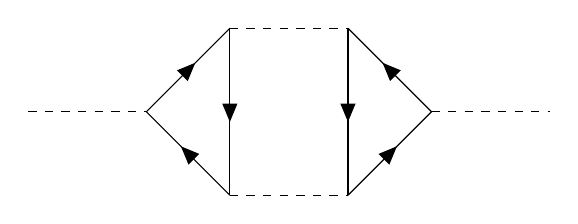
\begin{tikzpicture}
\begin{feynman}
\vertex (a);
\vertex[right=of a] (b);
\vertex[above right=of b] (l1);
\vertex[below right=of b] (l2);
\vertex[right=of l1] (l3);
\vertex[right=of l2] (l4);
\vertex[above right=of l4] (c);
\vertex[right=of c] (d);
\diagram* {
(a) -- [scalar] (b),
(b) -- [fermion] (l1) -- [fermion] (l2) -- [fermion] (b),
(l1) -- [scalar] (l3),
(l2) -- [scalar] (l4),
(c) -- [fermion] (l3) -- [fermion] (l4) -- [fermion] (c),
(c) -- [scalar] (d)
};
\end{feynman}
\end{tikzpicture}
\end{center}
at the three-loop level which is beyond the scope of our analysis. Therefore, a higher loop-order calculation would be necessary to probe the full structure of the muliparticle part of the dressed $\tilde{G}_{\psi}(p)$ propagator.  


\subsubsection{Evaluation of the $\phi$ One-Particle Irreducible Amplitude in the Case $m \ge 2 M$}

Now, we consider to the case $m > 2 M$. In this case, the $\phi$ meson is stable and thus asymptotic scattering $\phi$ states cannot be defined. This does not affect the current theory because we are not consider $S$ matrix elements corresponding to asymptotic $\phi$ states. We need to consider term,
\[ - i \Sigma_\phi(p^2) = - \frac{ig^2}{16 \pi^2}  \left[ \gamma_E + \log{\delta} + \int_{0}^{1} \d{x} \log{\left[ x(x-1)p^2 + M^2 - i \epsilon \right]} \right] - i c_3 \]
With the renormalization condition $\mathrm{Re}[\Sigma(p^2 = m^2)] = 0$. We have shown that there is a residual imaginary part at $p^2 = m^2$ given by,
\[\Im[\Sigma_\phi(p^2)] = \frac{g^2}{16 \pi^2} \mathrm{Im}\left[ \int_{0}^{1} \d{x} \log{\left[ x(x-1)p^2 + M^2 - i \epsilon \right]} \right] = -\frac{g^2}{16 \pi}
\begin{cases}
\sqrt{1 - \frac{4M^2}{p^2}} & m > 2M \\
0 & m \le 2M
\end{cases} \]
To satisfy the renormalization condition, following the above results we set,
\begin{align*}
c_3 & = - \frac{g^2}{16 \pi^2} \left[ \gamma_E + \log{\delta} + \int_0^1 \mathrm{Re}\left[ \log(x(x-1) m^2 + M^2 - i \epsilon) \right] \right] 
\\
&= - \frac{g^2}{16 \pi^2} \left[ \gamma_E + \log{\delta} + \sqrt{\frac{m^2 - 4 M^2}{m^2}} \log{\left[ \frac{\sqrt{\frac{m^2}{m^2 - 4 M^2}} + 1}{\sqrt{\frac{m^2}{m^2 - 4 M^2}} - 1} \right]} + 2( \log{M} - 1) \right]
\end{align*}
Therefore, we are interested in the quantity,
\[ - i \Sigma_\phi(p^2) = (-ig)^2 V(p) - i c_3 = - \frac{ig^2}{16 \pi^2} \left[ \int_{0}^{1} \d{x} \log{\left[\frac{x(x - 1) p^2 + M^2}{M^2} \right]} - \sqrt{\frac{m^2 - 4 M^2}{m^2}} \log{\left[ \frac{\sqrt{\frac{m^2}{m^2 - 4 M^2}} + 1}{\sqrt{\frac{m^2}{m^2 - 4 M^2}} - 1} \right]} + 2 \right] \]
Luckily, this integral is nearly identical to the one worked out above so I will mearly quote the result,
\begin{align*}
\Sigma_\phi(p^2) =
\frac{g^2}{16 \pi^2}
\begin{cases}
2 \sqrt{\frac{4 M^2 - p^2}{-p^2}} \mathrm{arctanh}{\left(\sqrt{\frac{-p^2}{4 M^2 - p^2}}\right)} - \sqrt{\frac{m^2 - 4 M^2}{m^2}} \log{\left[ \frac{\sqrt{\frac{m^2}{m^2 - 4 M^2}} + 1}{\sqrt{\frac{m^2}{m^2 - 4 M^2}} - 1} \right]} 
& p^2 < 0
\\
&
\\
2 \sqrt{\frac{4 M^2 - p^2}{p^2}} \arctan{\left( \sqrt{\frac{p^2}{4 M^2 - p^2}} \right)} - \sqrt{\frac{m^2 - 4 M^2}{m^2}} \log{\left[ \frac{\sqrt{\frac{m^2}{m^2 - 4 M^2}} + 1}{\sqrt{\frac{m^2}{m^2 - 4 M^2}} - 1} \right]}
& 0 < p^2 < 4 M^2 
\\
&
\\
\sqrt{\frac{p^2 - 4 M^2}{p^2}} \log{\left[ \frac{\sqrt{\frac{p^2}{p^2 - 4 M^2}} + 1}{\sqrt{\frac{p^2}{p^2 - 4 M^2}} - 1} \right]} 
- \sqrt{\frac{m^2 - 4 M^2}{m^2}} \log{\left[ \frac{\sqrt{\frac{m^2}{m^2 - 4 M^2}} + 1}{\sqrt{\frac{m^2}{m^2 - 4 M^2}} - 1} \right]} - i\pi \sqrt{1 - \frac{4 M^2}{p^2}}
& p^2 > 4 M^2
\end{cases}
\end{align*}
To calculate the residue, we need to find the derivative of the real part of $\Sigma_\phi$. We can take this derivative directly from the above formula in the region $p^2 > 4 M^2$ (since $m > 2 M$). We get,
\[ \deriv{\mathrm{Re}[\Sigma_\phi]}{p^2} = \frac{g^2 M^2}{8 \pi p^4} \sqrt{\frac{p^2}{p^2-4 M^2}} \log{\left[\frac{\sqrt{\frac{p^2}{p^2-4
   M^2}}+1}{\sqrt{\frac{p^2}{p^2-4 M^2}}-1}\right]} + \frac{g^2}{16 \pi p^2}  \]
Therefore, when $m > 2 M$, the residue in the dressed $\phi$ propagator can be written,
\[ Z_\phi = \left( 1 - \frac{g^2 M^2}{8 \pi m^4} \sqrt{\frac{m^2}{m^2-4 M^2}} \log{ \left[\frac{\sqrt{\frac{m^2}{m^2-4
   M^2}}+1}{\sqrt{\frac{m^2}{m^2-4 M^2}}-1}\right]} - \frac{g^2}{16 \pi m^2}  \right)^{-1} \]
As before, I will here define the field strength renomalized one-particle irreducible amplitude,
\begin{align*}
\Sigma_\phi^{renorm}(p^2) & = \Sigma_\phi(p^2) - (p^2 - m^2) \deriv{\mathrm{Re}[\Sigma_\phi]}{p^2} \bigg|_{p^2 = m^2} 
\end{align*}

\subsubsection{Discussion of the $\psi$ One-Particle Irreducible Amplitude}

For $\phi$ particles there is no need to seperately consider cases for the form of the two-point function. For all values of the parameters, $\Sigma_\psi(p^2 = M^2)$ is real the renormalization conditions can exactly fix $\Sigma_\psi(p^2 = M^2) = 0$. Therefore, the two-point function takes the form of a dressed propagator which can be considered in the assymptotic limit,
\[ \tilde{G}_\psi^{(2)}(p) = \frac{i Z}{p^2 - m^2 + i \epsilon} \]
This fact can directly be seen from the form of the integral, 
\[ - i \Sigma_\psi(m^2) = -\frac{ig^2}{16 \pi^2} \left[ \gamma_E + \log{\delta} + \int_{0}^{1} \d{x} \log{\left[ x m^2 + (1 - x)^2 M^2 \right]} \right] - i c_2 \]
in which, having taken $\epsilon \to 0$, the argument of the logarithm is clearly positive. Physically, the fact that $\Sigma_\phi(p^2 = M^2)$ is real is a reflection of the fact that $\phi$ particles must be stable due to the conservation of Noether charge. Since $\psi$ particles are the lowest mass excitation carrying Noether charge, the conservation law precludes $\psi$ decays which would have to end with a state of higher mass violating the conservation of energy. \bigskip\\
Although they are horrendous, the integrals determining $\Sigma_\psi$ can actually be explicitly computed. Luckily, since the form of these integrals is better behaved, there are fewer cases to consider. However, we will not actually need these integrals to compute the scattering cross section at this order so I will omit these details. All the important features can be read off from the pole structure of the integral,
\[ - i \Sigma_\psi(p^2) = - \frac{ig^2}{16 \pi^2} \left[ \int_{0}^{1} \d{x} \log{\left[\frac{ x(x - 1) p^2 + x m^2 + (1 - x) M^2}{x m^2 + (x - 1)^2 M^2} \right]} \right] \]
As discussd above, the denominator (and equivalently the counterterm) is real because $x m^2 + (1 - x)^2 M^2 \ge 0$. Consider the numerator which is the quadratic,
\[Q(x) = x(x - 1) p^2 + x m^2 + (1-x)M^2 = x^2 p^2 + x (m^2 - M^2 - p^2) + M^2 \]
First consider the case when $p^2 < 0$. Consider the endpoints $Q(0) = M^2$ and $Q(1) = p^2 + m^2 - M^2 - p^2 + M^2 = m^2$. Since both $Q(0) > 0$ and $Q(1) > 0$ and the parabola is convex down for $p^2 < 0$ we know that $Q(x) > 0$ for $x \in [0,1]$. Therefore, when $p^2 < 0$ the logarithm is real so $\Sigma_\psi$ is real and has no discontinuities. Furthermore, consider the case $p^2 > 0$. The discriminant of $Q$ is,
\[ (m^2 - M^2 - p^2)^2 - 4 M^2 p^2 = (p^2 - m^2 - M^2)^2 - 4 m^2 M^2 \]
However, 
\[ (p^2 - m^2 - M^2)^2 < 4 m^2 M^2 \iff - 2 m M < p^2 - m^2 - M^2 < 2 m M\]
which is equvalent to $(m - M)^2 < p^2 < (m + M)^2$. Therefore, $Q$ has real roots exactly when\[p^2 \in [0, (m - M)^2] \cup [(m+M)^2, \infty]\]
The maximum of this quadratic occurs at,
\[x_{max} = \frac{p^2 - m^2 + M^2}{2 p^2}  = \frac{1}{2} + \frac{M^2 - m^2}{2 p^2}\]
For the case $p^2 \in [0, (m - M)^2]$ this value satisfies,
\[ \left(x_{max} - \frac{1}{2} \right)^2 = \left( \frac{M^2 - m^2}{2 p^2} \right)^2 \ge \left( \frac{M^2 - m^2}{2 (M - m)^2} \right)^2 = \frac{1}{4} \left( \frac{M + m}{M - m} \right)^2  \ge \frac{1}{4}\]
Therefore, $x_{max} \notin [0, 1]$. However, since $Q(0) > 0$ and $Q(1) > 0$ if $Q(x) < 0$ for some $x \in [0, 1]$ then there would have to be a critical point in the range $[0, 1]$ which we have shown does not exist. Furthermore, if $p^2 > (m + M)^2$ then, 
\[ \left(x_{max} - \frac{1}{2} \right)^2 = \left( \frac{M^2 - m^2}{2 p^2} \right)^2 \le \left( \frac{M^2 - m^2}{2 (M + m)^2} \right)^2 = \frac{1}{4} \left( \frac{M - m}{M + m} \right)^2  \le \frac{1}{4}\]
Therefore, $x_{min} \in [0, 1]$ and since we know that $Q$ has a real root but has positive end behavior we must have $Q(x_{max}) < 0$ and thus the integrand becomes complex in this case. \bigskip\\
In summary, for $p^2 < (m + M)^2$ the function $\Sigma_{\psi}$ is real. For $p^2 \ge (m + M)^2$, there is a branch cut in the logarithm and $\Sigma_\psi$ picks up a imaginary part. Physically, this corresponds exactly to then energy needed to produce a two particle $\psi \phi$ state which is the lowest energy multiparticle state with Noether charge $1$. If $\Sigma_\psi(p^2)$ is viewed as a function of a complex variable then it has a branch cut starting at $p^2 = (m + M)^2$ due to the sign dependence of the imaginary part under the change $i \epsilon \to - i \epsilon$ in the integral. This brach cut again exactly corresponds to the mulitparticle continuum predicted by the K{\"a}ll{\'e}n-Lehmann spectral representation.

\subsection{Center of Mass Frame Calculations}

Although we have computed a valid expression for the scattering cross section, it is not much use without further simplifications. First, notice that the reduced vertex function only appears with on-shell momentum arguments. Therefore, we can simplyfy,
\[\tilde{\Gamma}_{on-shell}(p_1, p_2) = \frac{ g^2}{16 \pi^2} \left[ \int_0^1 \frac{\d{x} \d{y} \d{z} \delta(x + y + z - 1)}{(y p_1 - z p_2)^2 + x m^2 - i \epsilon} - \int_0^1 \frac{\d{x} \d{y} \d{z} \delta(x + y + z - 1)}{(y - z)^2 M^2 + x m^2} \right]\]
The next simplification comes from the facts of two particle scattering in the center of mass frame. In this reference frame, we can write our four momentum fourvectors as,
\[ p_1 = (E, \vec{p}) \quad p_2 = (E, -\vec{p}) \quad p_1' = (E, \vec{p'}) \quad p_2' = (E, -\vec{p'}) \]
With this parametrization, the Mandelstam paramters become,
\[ s = (p_1 + p_2)^2 = 4 E^2 \quad t = (p_1 - p_1')^2 = -2 \vec{p}^{\, 2} (1 - \cos{\Theta}) \quad u = (p_1 - p_2')^2 = -2 \vec{p}^{\, 2} (1 + \cos{\Theta}) \]
Now we need to simplify the eight integrals,
\begin{align*} 
\tilde{\Gamma}_{on-shell}(p_1, p_2) &= \frac{g^2}{16 \pi^2} \int_0^1 \frac{\d{x} \d{y} \d{z} \delta(x + y + z - 1)}{(y - z)^2 E^2 - (y + z)^2 \vec{p}^{\, 2} + x m^2 - i \epsilon} + c_4
\\
& = \frac{g^2}{16 \pi^2} \int_0^1 \frac{\d{x} \d{y} \d{z} \delta(x + y + z - 1) }{(y - z)^2 (M^2 + \vec{p}^{\, 2}) - (y + z)^2 \vec{p}^{\, 2} + x m^2 - i \epsilon} + c_4
\\
& = \frac{g^2}{16 \pi^2} \int_0^1 \frac{ \d{x} \d{y} \d{z} \delta(x + y + z - 1) }{(y + z)^2 M^2 - yz s + x m^2 - i \epsilon} + c_4
\end{align*}
Denote this function as $\tilde{\Gamma}(s)$.
Similarly, $\tilde{\Gamma}(p_1', p_2') = \tilde{\Gamma}(s)$ since the integral is expressed only in terms of rotationally invariant quantities and $(p_1', p_2')$ is a rotation of $(p_1, p_2)$ through the scattering angle.
Next, we need to calculate, 
\begin{align*} 
\tilde{\Gamma}_{on-shell}(p_1, -p_1') &= \frac{g^2}{16 \pi^2} \int_0^1 \frac{\d{x} \d{y} \d{z} \delta(x + y + z - 1)}{(y + z)^2 (M^2 + \vec{p}^{\, 2}) - (y^2 + z^2 + 2 yz \cos{\Theta}) \vec{p}^{\, 2}+ x m^2 - i \epsilon} + c_4 
\\
& = \frac{g^2}{16 \pi^2} \int_0^1 \frac{\d{x} \d{y} \d{z} \delta(x + y + z - 1)}{(y + z)^2 M^2 + 2yz(1 - \cos{\Theta})\vec{p}^{\, 2} + x m^2 - i \epsilon}
\\
& = \frac{g^2}{16 \pi^2} \int_0^1 \frac{\d{x} \d{y} \d{z} \delta(x + y + z - 1) }{(y + z)^2M^2 - yz t + x m^2 - i \epsilon} + c_4
\end{align*}
This is the same function $\tilde{\Gamma}(t)$ simply with $s$ replaced with $u$. Similarly, $\tilde{\Gamma}(p_2, p_2') = \tilde{\Gamma}(t)$ because this integral is invariant under partiy inversion and $(p_2, p_2')$ is a inversion through the center of mass of $(p_1, p_1')$.
All the vertex functions can be expressed in terms of a single function $\tilde{\Gamma}(\alpha)$ which is plotted below. This function represents the dependence of the effective coupling constant on the scattering energy.

\begin{figure}[!htb]
    \centering
    \begin{minipage}[b]{.45\textwidth}
        \centering
        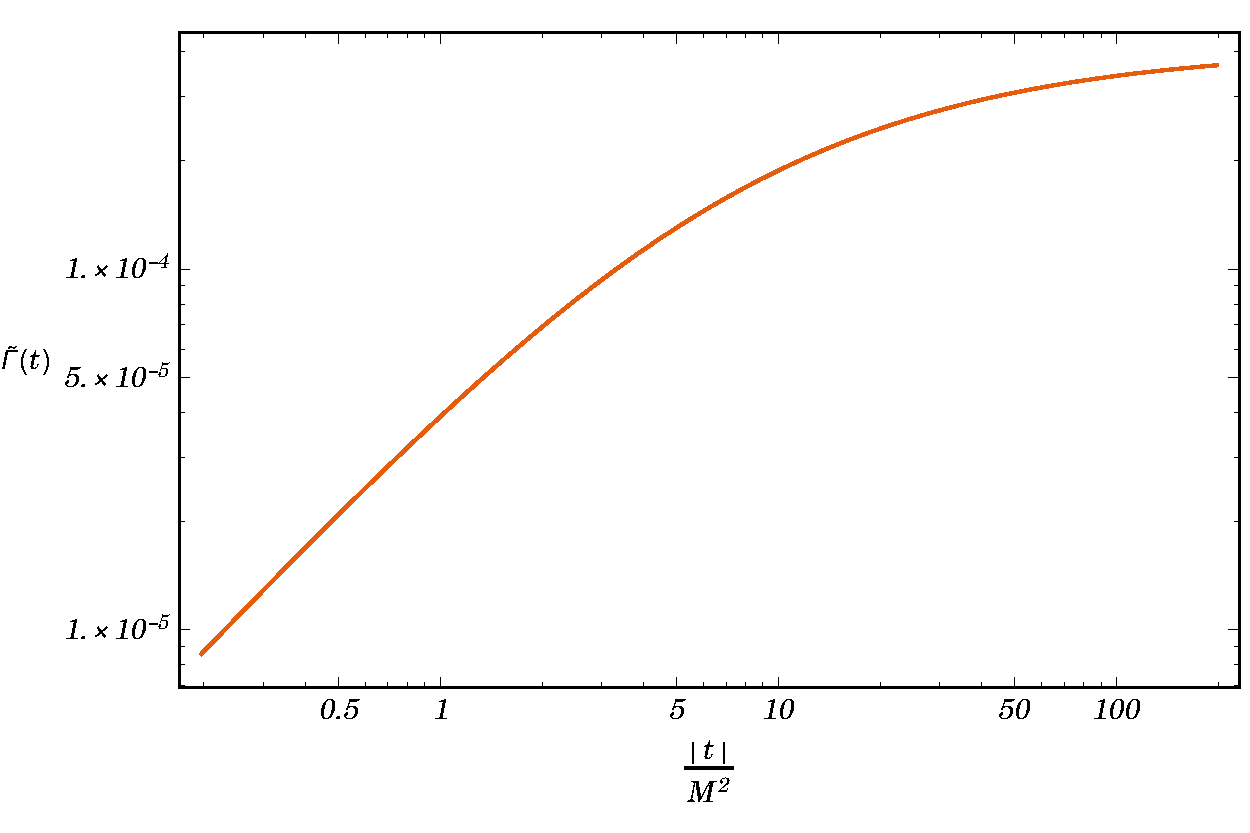
\includegraphics[width=9cm, height=7cm]	{Gamma-t-channel}
        \caption{The absolute value of the reduced vertex Function $\tilde{\Gamma}(t)$ for the $t$-channel process in the stable meson regime using parameters $m = 0.5M$ and $g = 0.25M$.}
        \label{fig:gamma1}
    \end{minipage}%
    \hfill
    \begin{minipage}[b]{0.45\textwidth}
        \centering
        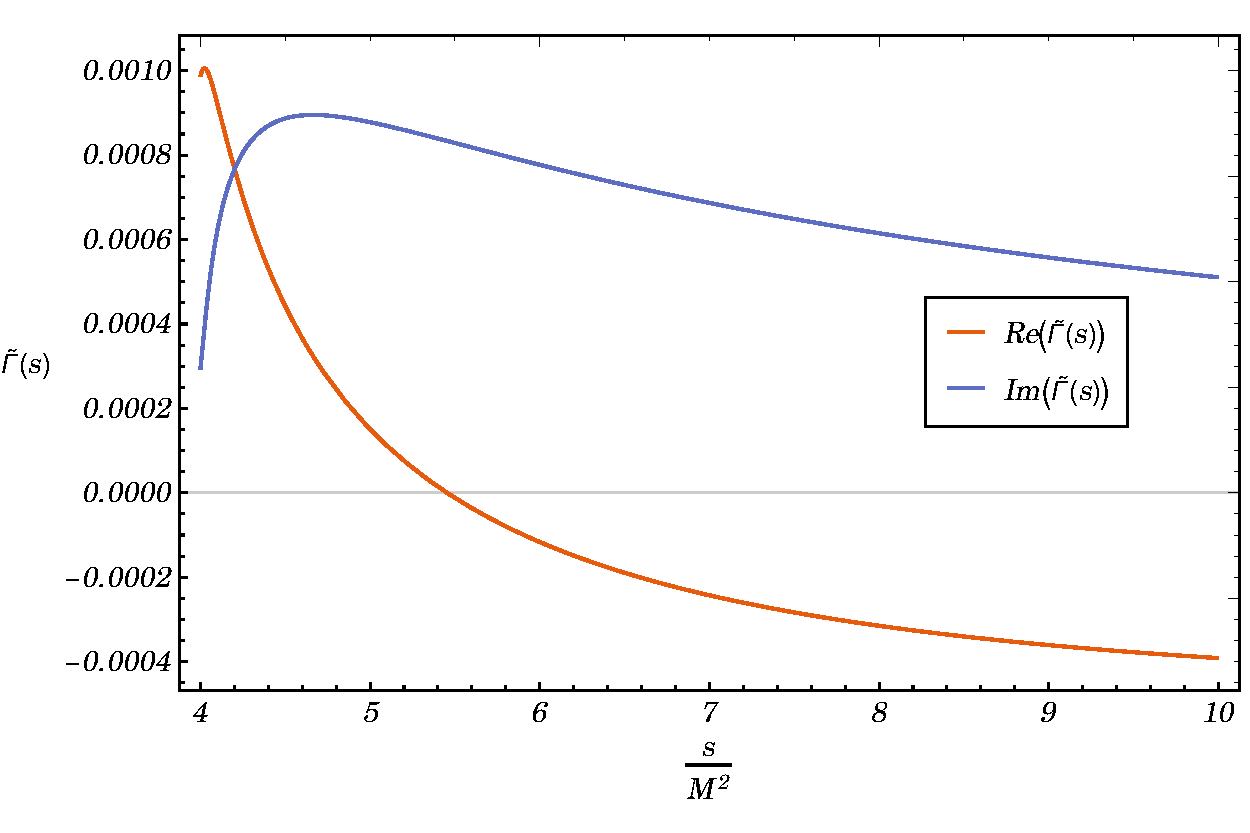
\includegraphics[width=9cm, height=7cm]{Gamma-s-channel}
        \caption{The reduced vertex Function $\tilde{\Gamma}(t)$ for the $s$-channel process in the stable meson regime using parameters $m = 0.5M$ and $g = 0.25M$.}
        \label{fig:gamma1}
    \end{minipage}
\end{figure}

\begin{figure}[!htb]
    \centering
    \begin{minipage}[b]{.45\textwidth}
        \centering
        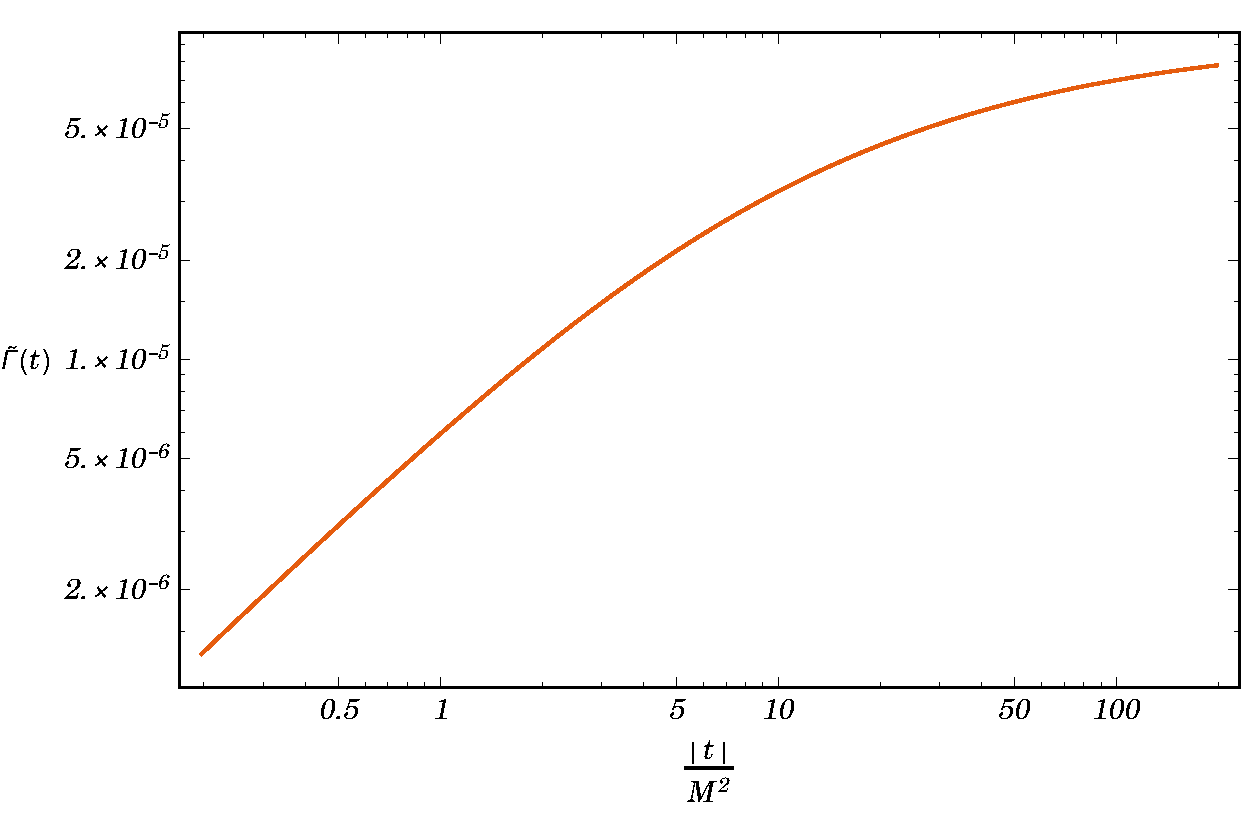
\includegraphics[width=9cm, height=7cm]	{Gamma-t-channel-unstable}
        \caption{The absolute value of the reduced vertex Function $\tilde{\Gamma}(t)$ for the $t$-channel process in the unstable meson regime using parameters $m = 2.5M$ and $g = 0.25M$.}
        \label{fig:gamma1}
    \end{minipage}%
    \hfill
    \begin{minipage}[b]{0.45\textwidth}
        \centering
        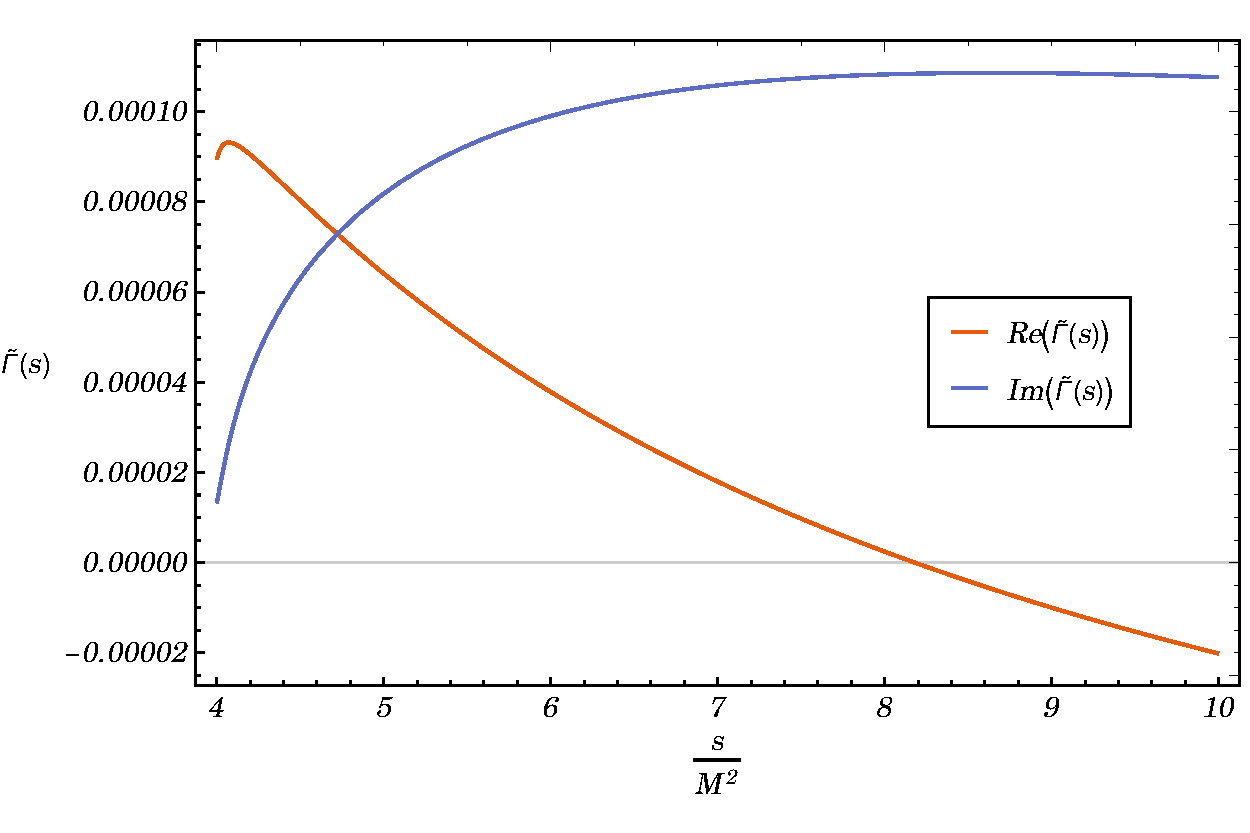
\includegraphics[width=9cm, height=7cm]{Gamma-s-channel-unstable}
        \caption{The reduced vertex Function $\tilde{\Gamma}(t)$ for the $s$-channel process in the unstable meson regime using parameters $m = 2.5M$ and $g = 0.25M$.}
        \label{fig:gamma1}
    \end{minipage}
\end{figure}

Now we need to calculate the box diagram integrals,
\begin{align*}  
i\mathcal{M}_B(p_1, p_2, p_1', p_2') &= \frac{ig^4}{16 \pi^2} \int_{0}^{1} \frac{\d{x} \d{y} \d{z} \d{w} \delta(x + y + z + w - 1) }{[(y p_1 + z (p_1 + p_2) + w p_1' )^2 - z (p_1 + p_2)^2 + (x + z)m^2 - i \epsilon]^2} 
\\
& = \frac{ig^4}{16 \pi^2} \int_{0}^{1} \frac{\d{x} \d{y} \d{z} \d{w} \delta(x + y + z + w - 1) }{[(y + 2 z + w)^2 (M^2 + \vec{p}^{\, 2}) - \vec{p}^{\, 2}(y^2 + w^2 + 2 yw \cos{\Theta}) - z s + (x + z)m^2 - i \epsilon]^2} 
\\
& = \frac{ig^4}{16 \pi^2} \int_{0}^{1} \frac{\d{x} \d{y} \d{z} \d{w} \delta(x + y + z + w - 1) }{[M^2 (y + w)^2 - yw t + (y + w)z s + (z^2 - z)s + (x + z)m^2 - i \epsilon]^2} 
\end{align*}
similarly,
\begin{align*}  
i\mathcal{M}_B(p_1, -p_1', -p_2, p_2') & = \frac{ig^4}{16 \pi^2} \int_{0}^{1} \frac{\d{x} \d{y} \d{z} \d{w} \delta(x + y + z + w - 1) }{[M^2 (y + w)^2 - yw s + (y + w)z t + (z^2 - z) t + (x + z)m^2 - i \epsilon]^2} 
\\
i\mathcal{M}_B(p_1, p_2, p_2', p_1') & = \frac{ig^4}{16 \pi^2} \int_{0}^{1} \frac{\d{x} \d{y} \d{z} \d{w} \delta(x + y + z + w - 1) }{[M^2 (y + w)^2 - yw u + (y + w)z s + (z^2 - z) s + (x + z)m^2 - i \epsilon]^2} 
\\
i\mathcal{M}_B(p_1, -p_1', p_2', -p_2) & = \frac{ig^4}{16 \pi^2} \int_{0}^{1} \frac{\d{x} \d{y} \d{z} \d{w} \delta(x + y + z + w - 1) }{[M^2 (y + w)^2 - yw u + (y + w)z t + (z^2 - z) t + (x + z)m^2 - i \epsilon]^2} 
\end{align*}
Therefore, these three integrals are all expressible in terms of a single function,
\[ B(a,b) = -\frac{g^2}{16 \pi^2} \int_{0}^{1} \frac{\d{x} \d{y} \d{z} \d{w} \delta(x + y + z + w - 1) }{[M^2 (y + w)^2 - yw a + (y + w)z b + (z^2 - z) b + (x + z)m^2 - i \epsilon]^2} \]
In terms of this function,
\begin{align*}
(-ig)^2 B(t, s) &= \mathcal{M}_B(p_1, p_2, p_1', p_2') \\
(-ig)^2 B(s, t) &= \mathcal{M}_B(p_1, -p_1', -p_2, p_2') \\
(-ig)^2 B(u, s) &= \mathcal{M}_B(p_1, p_2, p_2', p_1') \\
(-ig)^2 B(u, t) &= \mathcal{M}_B(p_1, -p_1', p_2', -p_2) 
\end{align*}
Therefore,
\[\mathcal{M}_{box} = (-ig)^2[B(t, s) + B(s, t) + B(u, s) + B(u,t)]\]
The $B$ integral must be computed numerically.
Now we have all the tools to evaluate the explict scattering cross section in the center of mass reference frame. In terms of these new functions,
\begin{align*}
\deriv{\sigma}{\Omega} 
&= \frac{g^4}{64 \pi^2 s} \left| \frac{i}{t - m^2} + \frac{i}{s - m^2} + \frac{2i \tilde{\Gamma}(s)}{s - m^2} + \frac{2i \tilde{\Gamma}(t)}{t - m^2} + \frac{i \Sigma_\phi(t)}{(t - m^2)^2} + \frac{i \Sigma_\phi(s)}{(s - m^2)^2} + i B(t, s) + i B(s, t) + i B(u, s) + i B(u,t)  \right|^2 
\end{align*}

\subsection{Taming Resonance Poles in the Scattering Cross Section}

In the case $m > 2M$ then $s = m^2 > 4 M^2$ is a valid scattering energy and thus there is an uphysical pole in the scattering cross section due to the propagator $\frac{i}{s - m^2}$. However, this pole exists exactly when $\phi$ becomes unstable. This is because if $\phi$ mesons can be produced in scattering experiments then, by time reversal symmetry, $\phi$ must be able to decay and so much be unstable. The theory is saved by the fact that an unstable meson shifts the poles of the exact propagator off the real axis. This pole persists to every order in perturbation theory but is absent from the exact theory. To correct this failing of the perturbative approach, we can replace the terms,
\[ \frac{i}{s - m^2} + \frac{i \Sigma_\phi(s)}{(s - m^2)^2} \quad \text{and} \quad \frac{i}{t - m^2} + \frac{i \Sigma_\phi(t)}{(t - m^2)^2} \]
with the exact two-point function i.e. dressed $\phi$ propagators,
\[ \frac{i}{s - m^2 - \Sigma_\phi(s)} \quad \text{and} \quad \frac{i}{t - m^2 - \Sigma_\phi(t)}\]
The terms we have calculated at the one-loop level correspond to the first nontrivial term in the geometric sequence for the exact propagator.
Diagramatically, this is equivalent to including the following terms above the one-loop level,
\begin{equation*}
\begin{tikzpicture}[baseline = -0.11cm]
\begin{feynman}
\vertex (a);
\vertex [above left=of a, momentum = $p_1$] (i1) ;
\vertex [below left=of a, rmomentum = $p_2$] (i2) 
;
\vertex [right=of a, blob] (b) {\(\mathbf{1PI}\)};
\vertex [right=of b] (c);
\vertex [above right=of c] (f1) ;
\vertex [below right=of c] (f2) ;
\diagram* {
(i1) --[fermion, momentum = $p_1$] (a) -- [fermion, rmomentum = $p_2$] (i2),
(a) -- [scalar] (b) -- [scalar] (c)
(f2) --[fermion, rmomentum = $p_1'$] (c) -- [fermion, momentum = $p_2'$] (f1)
};
\end{feynman}
\end{tikzpicture}
\quad 
+
\quad 
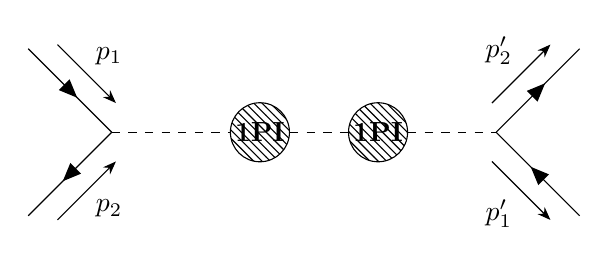
\begin{tikzpicture}[baseline = -0.11cm]
\begin{feynman}
\vertex (a);
\vertex [above left=of a, momentum = $p_1$] (i1) ;
\vertex [below left=of a, rmomentum = $p_2$] (i2) ;
\vertex [right=of a, blob] (b) {\(\mathbf{1PI}\)};
\vertex [right=of b, blob] (c) {\(\mathbf{1PI}\)};
\vertex [right=of c] (d);
\vertex [above right=of d] (f1) ;
\vertex [below right=of d] (f2) ;
\diagram* {
(i1) --[fermion, momentum = $p_1$] (a) -- [fermion, rmomentum = $p_2$] (i2),
(a) -- [scalar] (b) -- [scalar] (c) -- [scalar] (d),
(f2) --[fermion, rmomentum = $p_1'$] (d) -- [fermion, momentum = $p_2'$] (f1)
};
\end{feynman}
\end{tikzpicture}
\end{equation*}
\begin{equation*}
\quad 
+
\quad 
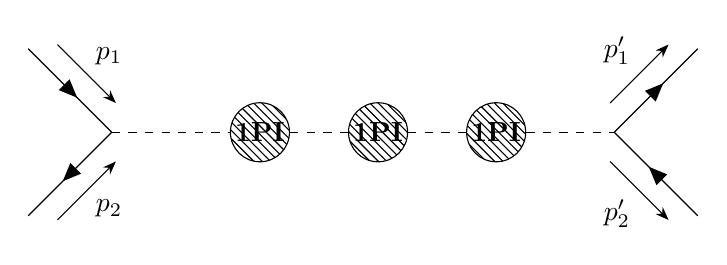
\begin{tikzpicture}[baseline = -0.11cm]
\begin{feynman}
\vertex (a);
\vertex [above left=of a] (i1) ;
\vertex [below left=of a] (i2) ;
\vertex [right=of a, blob] (b) {\(\mathbf{1PI}\)};
\vertex [right=of b, blob] (c) {\(\mathbf{1PI}\)};
\vertex [right=of c, blob] (d) {\(\mathbf{1PI}\)};
\vertex [right=of d] (e);
\vertex [above right=of e] (f1) ;
\vertex [below right=of e] (f2) ;
\diagram* {
(i1) --[fermion, momentum = $p_1$] (a) -- [fermion, rmomentum = $p_2$] (i2),
(a) -- [scalar] (b) -- [scalar] (c) -- [scalar] (d) -- [scalar] (e),
(f2) --[fermion, rmomentum = $p_2'$] (e) -- [fermion, momentum = $p_1'$] (f1)
};
\end{feynman}
\end{tikzpicture}
\quad
+ 
\quad
\cdots
\end{equation*}
and similarly,
\begin{equation*}
\begin{tikzpicture}[baseline = -1.7cm]
\begin{feynman}
\vertex (a);
\vertex [above left=of a, momentum' = $p_1$] (i1) ;
\vertex [above right=of a, rmomentum = $p_2$] (i2) 
;
\vertex [below=of a, blob] (b) {\(\mathbf{1PI}\)};
\vertex [below=of b] (c);
\vertex [below left=of c] (f1) ;
\vertex [below right=of c] (f2) ;
\diagram* {
(i1) --[fermion, momentum' = $p_1$] (a) -- [fermion, momentum' = $p_1'$] (i2),
(a) -- [scalar] (b) -- [scalar] (c)
(f2) --[fermion, rmomentum' = $p_2'$] (c) -- [fermion, rmomentum' = $p_2$] (f1)
};
\end{feynman}
\end{tikzpicture}
\quad 
+
\quad 
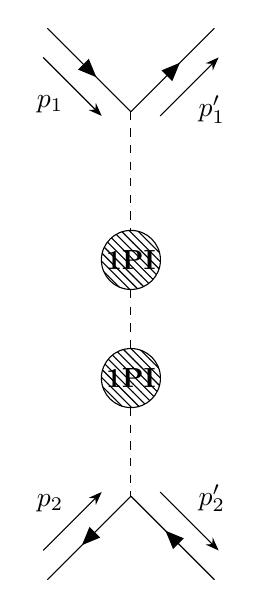
\begin{tikzpicture}[baseline = -2.5cm]
\begin{feynman}
\vertex (a);
\vertex [above left=of a, momentum' = $p_1$] (i1) ;
\vertex [above right=of a, rmomentum = $p_2$] (i2) 
;
\vertex [below=of a, blob] (b) {\(\mathbf{1PI}\)};
\vertex [below=of b, blob] (c) {\(\mathbf{1PI}\)};
\vertex [below=of c] (d);
\vertex [below left=of d] (f1) ;
\vertex [below right=of d] (f2) ;
\diagram* {
(i1) --[fermion, momentum' = $p_1$] (a) -- [fermion, momentum' = $p_1'$] (i2),
(a) -- [scalar] (b) -- [scalar] (c) -- [scalar] (d),
(f2) --[fermion, rmomentum' = $p_2'$] (d) -- [fermion, rmomentum' = $p_2$] (f1)
};
\end{feynman}
\end{tikzpicture}
\quad 
+
\quad 
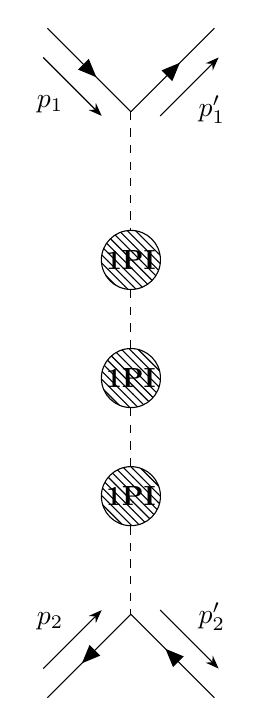
\begin{tikzpicture}[baseline = -3.2cm]
\begin{feynman}
\vertex (a);
\vertex [above left=of a, momentum' = $p_1$] (i1) ;
\vertex [above right=of a, rmomentum = $p_2$] (i2) 
;
\vertex [below=of a, blob] (b) {\(\mathbf{1PI}\)};
\vertex [below=of b, blob] (c) {\(\mathbf{1PI}\)};
\vertex [below=of c, blob] (d) {\(\mathbf{1PI}\)};
\vertex [below=of d] (e);
\vertex [below left=of e] (f1) ;
\vertex [below right=of e] (f2) ;
\diagram* {
(i1) --[fermion, momentum' = $p_1$] (a) -- [fermion, momentum' = $p_1'$] (i2),
(a) -- [scalar] (b) -- [scalar] (c) -- [scalar] (d) -- [scalar] (e),
(f2) --[fermion, rmomentum' = $p_2'$] (e) -- [fermion, rmomentum' = $p_2$] (f1)
};
\end{feynman}
\end{tikzpicture}
\quad
+ 
\quad
\cdots
\end{equation*}
and summing the geometric series analogously to how the exact propagator is derived. To fully remove this pole in the scattering cross section, we should also replace the terms,
\[ \frac{2i \tilde{\Gamma}(s)}{s - m^2} \quad \frac{2i \tilde{\Gamma}(t)}{t - m^2} \]
with the terms using the full propagator,
\[ \frac{2i \tilde{\Gamma}(s)}{s - m^2 - \Sigma_\phi(s)} \quad \frac{2i \tilde{\Gamma}(t)}{t - m^2 - \Sigma_\phi(t)} \]
which diagramatically correspond to the higher-loop terms,
\begin{equation*}
\begin{tikzpicture}[baseline = -0.11cm]
\begin{feynman}
\vertex [blob](a) {\(\Gamma\)};
\vertex [above left=of a, momentum = $p_1$] (i1) ;
\vertex [below left=of a, rmomentum = $p_2$] (i2) 
;
\vertex [right=of a, blob] (b) {\(\mathbf{1PI}\)};
\vertex [right=of b] (c);
\vertex [above right=of c] (f1) ;
\vertex [below right=of c] (f2) ;
\diagram* {
(i1) --[fermion, momentum = $p_1$] (a) -- [fermion, rmomentum = $p_2$] (i2),
(a) -- [scalar] (b) -- [scalar] (c)
(f2) --[fermion, rmomentum = $p_1'$] (c) -- [fermion, momentum = $p_2'$] (f1)
};
\end{feynman}
\end{tikzpicture}
\quad 
+
\quad 
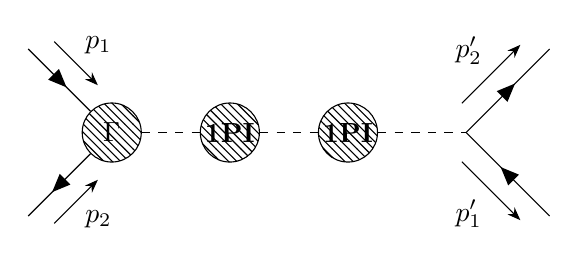
\begin{tikzpicture}[baseline = -0.11cm]
\begin{feynman}
\vertex [blob](a) {\(\Gamma\)};
\vertex [above left=of a, momentum = $p_1$] (i1) ;
\vertex [below left=of a, rmomentum = $p_2$] (i2) ;
\vertex [right=of a, blob] (b) {\(\mathbf{1PI}\)};
\vertex [right=of b, blob] (c) {\(\mathbf{1PI}\)};
\vertex [right=of c] (d);
\vertex [above right=of d] (f1) ;
\vertex [below right=of d] (f2) ;
\diagram* {
(i1) --[fermion, momentum = $p_1$] (a) -- [fermion, rmomentum = $p_2$] (i2),
(a) -- [scalar] (b) -- [scalar] (c) -- [scalar] (d),
(f2) --[fermion, rmomentum = $p_1'$] (d) -- [fermion, momentum = $p_2'$] (f1)
};
\end{feynman}
\end{tikzpicture}
\end{equation*}
\begin{equation*}
\quad 
+
\quad 
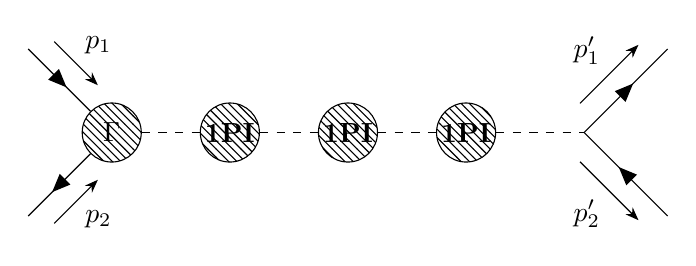
\begin{tikzpicture}[baseline = -0.11cm]
\begin{feynman}
\vertex [blob](a) {\(\Gamma\)};
\vertex [above left=of a] (i1) ;
\vertex [below left=of a] (i2) ;
\vertex [right=of a, blob] (b) {\(\mathbf{1PI}\)};
\vertex [right=of b, blob] (c) {\(\mathbf{1PI}\)};
\vertex [right=of c, blob] (d) {\(\mathbf{1PI}\)};
\vertex [right=of d] (e);
\vertex [above right=of e] (f1) ;
\vertex [below right=of e] (f2) ;
\diagram* {
(i1) --[fermion, momentum = $p_1$] (a) -- [fermion, rmomentum = $p_2$] (i2),
(a) -- [scalar] (b) -- [scalar] (c) -- [scalar] (d) -- [scalar] (e),
(f2) --[fermion, rmomentum = $p_2'$] (e) -- [fermion, momentum = $p_1'$] (f1)
};
\end{feynman}
\end{tikzpicture}
\quad
+ 
\quad
\cdots
\end{equation*}
and similarly,
\begin{equation*}
\begin{tikzpicture}[baseline = -1.7cm]
\begin{feynman}
\vertex [blob](a) {\(\Gamma\)};
\vertex [above left=of a, momentum' = $p_1$] (i1) ;
\vertex [above right=of a, rmomentum = $p_2$] (i2) 
;
\vertex [below=of a, blob] (b) {\(\mathbf{1PI}\)};
\vertex [below=of b] (c);
\vertex [below left=of c] (f1) ;
\vertex [below right=of c] (f2) ;
\diagram* {
(i1) --[fermion, momentum' = $p_1$] (a) -- [fermion, momentum' = $p_1'$] (i2),
(a) -- [scalar] (b) -- [scalar] (c)
(f2) --[fermion, rmomentum' = $p_2'$] (c) -- [fermion, rmomentum' = $p_2$] (f1)
};
\end{feynman}
\end{tikzpicture}
\quad 
+
\quad 
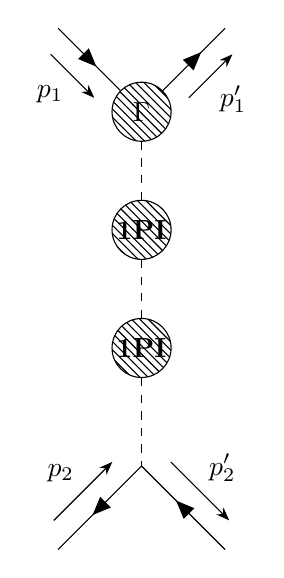
\begin{tikzpicture}[baseline = -2.5cm]
\begin{feynman}
\vertex [blob](a) {\(\Gamma\)};
\vertex [above left=of a, momentum' = $p_1$] (i1) ;
\vertex [above right=of a, rmomentum = $p_2$] (i2) 
;
\vertex [below=of a, blob] (b) {\(\mathbf{1PI}\)};
\vertex [below=of b, blob] (c) {\(\mathbf{1PI}\)};
\vertex [below=of c] (d);
\vertex [below left=of d] (f1) ;
\vertex [below right=of d] (f2) ;
\diagram* {
(i1) --[fermion, momentum' = $p_1$] (a) -- [fermion, momentum' = $p_1'$] (i2),
(a) -- [scalar] (b) -- [scalar] (c) -- [scalar] (d),
(f2) --[fermion, rmomentum' = $p_2'$] (d) -- [fermion, rmomentum' = $p_2$] (f1)
};
\end{feynman}
\end{tikzpicture}
\quad 
+
\quad 
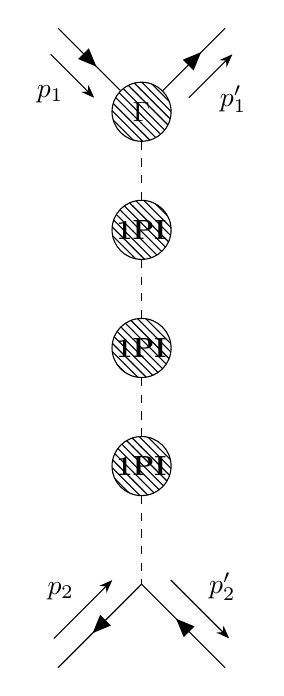
\begin{tikzpicture}[baseline = -3cm]
\begin{feynman}
\vertex [blob](a) {\(\Gamma\)};
\vertex [above left=of a, momentum' = $p_1$] (i1) ;
\vertex [above right=of a, rmomentum = $p_2$] (i2) 
;
\vertex [below=of a, blob] (b) {\(\mathbf{1PI}\)};
\vertex [below=of b, blob] (c) {\(\mathbf{1PI}\)};
\vertex [below=of c, blob] (d) {\(\mathbf{1PI}\)};
\vertex [below=of d] (e);
\vertex [below left=of e] (f1) ;
\vertex [below right=of e] (f2) ;
\diagram* {
(i1) --[fermion, momentum' = $p_1$] (a) -- [fermion, momentum' = $p_1'$] (i2),
(a) -- [scalar] (b) -- [scalar] (c) -- [scalar] (d) -- [scalar] (e),
(f2) --[fermion, rmomentum' = $p_2'$] (e) -- [fermion, rmomentum' = $p_2$] (f1)
};
\end{feynman}
\end{tikzpicture}
\quad
+ 
\quad
\cdots
\end{equation*}
and likewise flipped diagrams.
These corrections are at a higher order than the level of perturbation theory we are considering so there is no mystery in the fact that none of the these diagrams contributing to the expression with the full propagator appeared in our analysis.
Consider the real and imaginary parts of the propagator,
\begin{align*}
\tilde{G}^{(2)}(p) = \frac{i}{p^2 - m^2 - \mathrm{Re}[\Sigma(p^2)] - i \mathrm{Im}[\Sigma(p^2)]} = \frac{i(p^2 - m^2 - \mathrm{Re}[\Sigma(p^2)] + i \mathrm{Im}[\Sigma(p^2)])}{(p^2 - m^2 - \mathrm{Re}[\Sigma(p^2)])^2 + \mathrm{Im}[\Sigma(p^2)]^2}
\end{align*}
Therefore, at the resonant mass $p^2 = m^2$, since the renormalization condition implies $\mathrm{Re}[\Sigma(p^2 = m^2)] = 0$ then,
\[ \tilde{G}^{(2)}(p^2 = m^2) = - \frac{1}{\mathrm{Im}[\Sigma(m^2)]} = \frac{1}{m \Gamma} \]
Therefore, $\Gamma^{-1}$ measures the height of the reasonant peak, $2 \Gamma$ measures the full width at half max of the reasonant peak, and $\Gamma^{-1}$ gives the timetime of the unstable particle.
Using this notation, the scattering cross section becomes, 
\begin{align*}
\deriv{\sigma}{\Omega} 
&= \frac{g^4}{64 \pi^2 s} \left| \frac{1 + 2\tilde{\Gamma}(t)}{t - m^2 - \Sigma_\phi(t)} + \frac{1 + 2\tilde{\Gamma}(s)}{s - m^2 - \Sigma_\phi(s)} + B(t, s) + B(s, t) + B(u, s) + B(u, t)  \right|^2 
\end{align*}

\subsection{Explicit Evaluation of the Scattering Cross Section}

\subsubsection{Scattering in the Stable Meson Regime: $m < 2 M$}
Throughout this section, we will quote results for the case, $m = 0.5M$ and $g = 0.25$ in which the meson is stable. Results for the tree-level calculation which is accurate to order $g^4$ in the cross section and the one-loop calculation accurate to order $g^8$ in the cross section will be compared. In general, high energy scattering in enhanced at the one-loop level due to the contribution of the box diagrams, see figure \ref{StabHighEnergy}. The angular dependence of the scattering amplitude is presented as a magnitude-angle plot, see figure \ref{stable-angular}. which shows the dominance of forward scattering at high energy and little angular bias and low energy.

\begin{figure}
\begin{center}
\vspace*{-2cm}
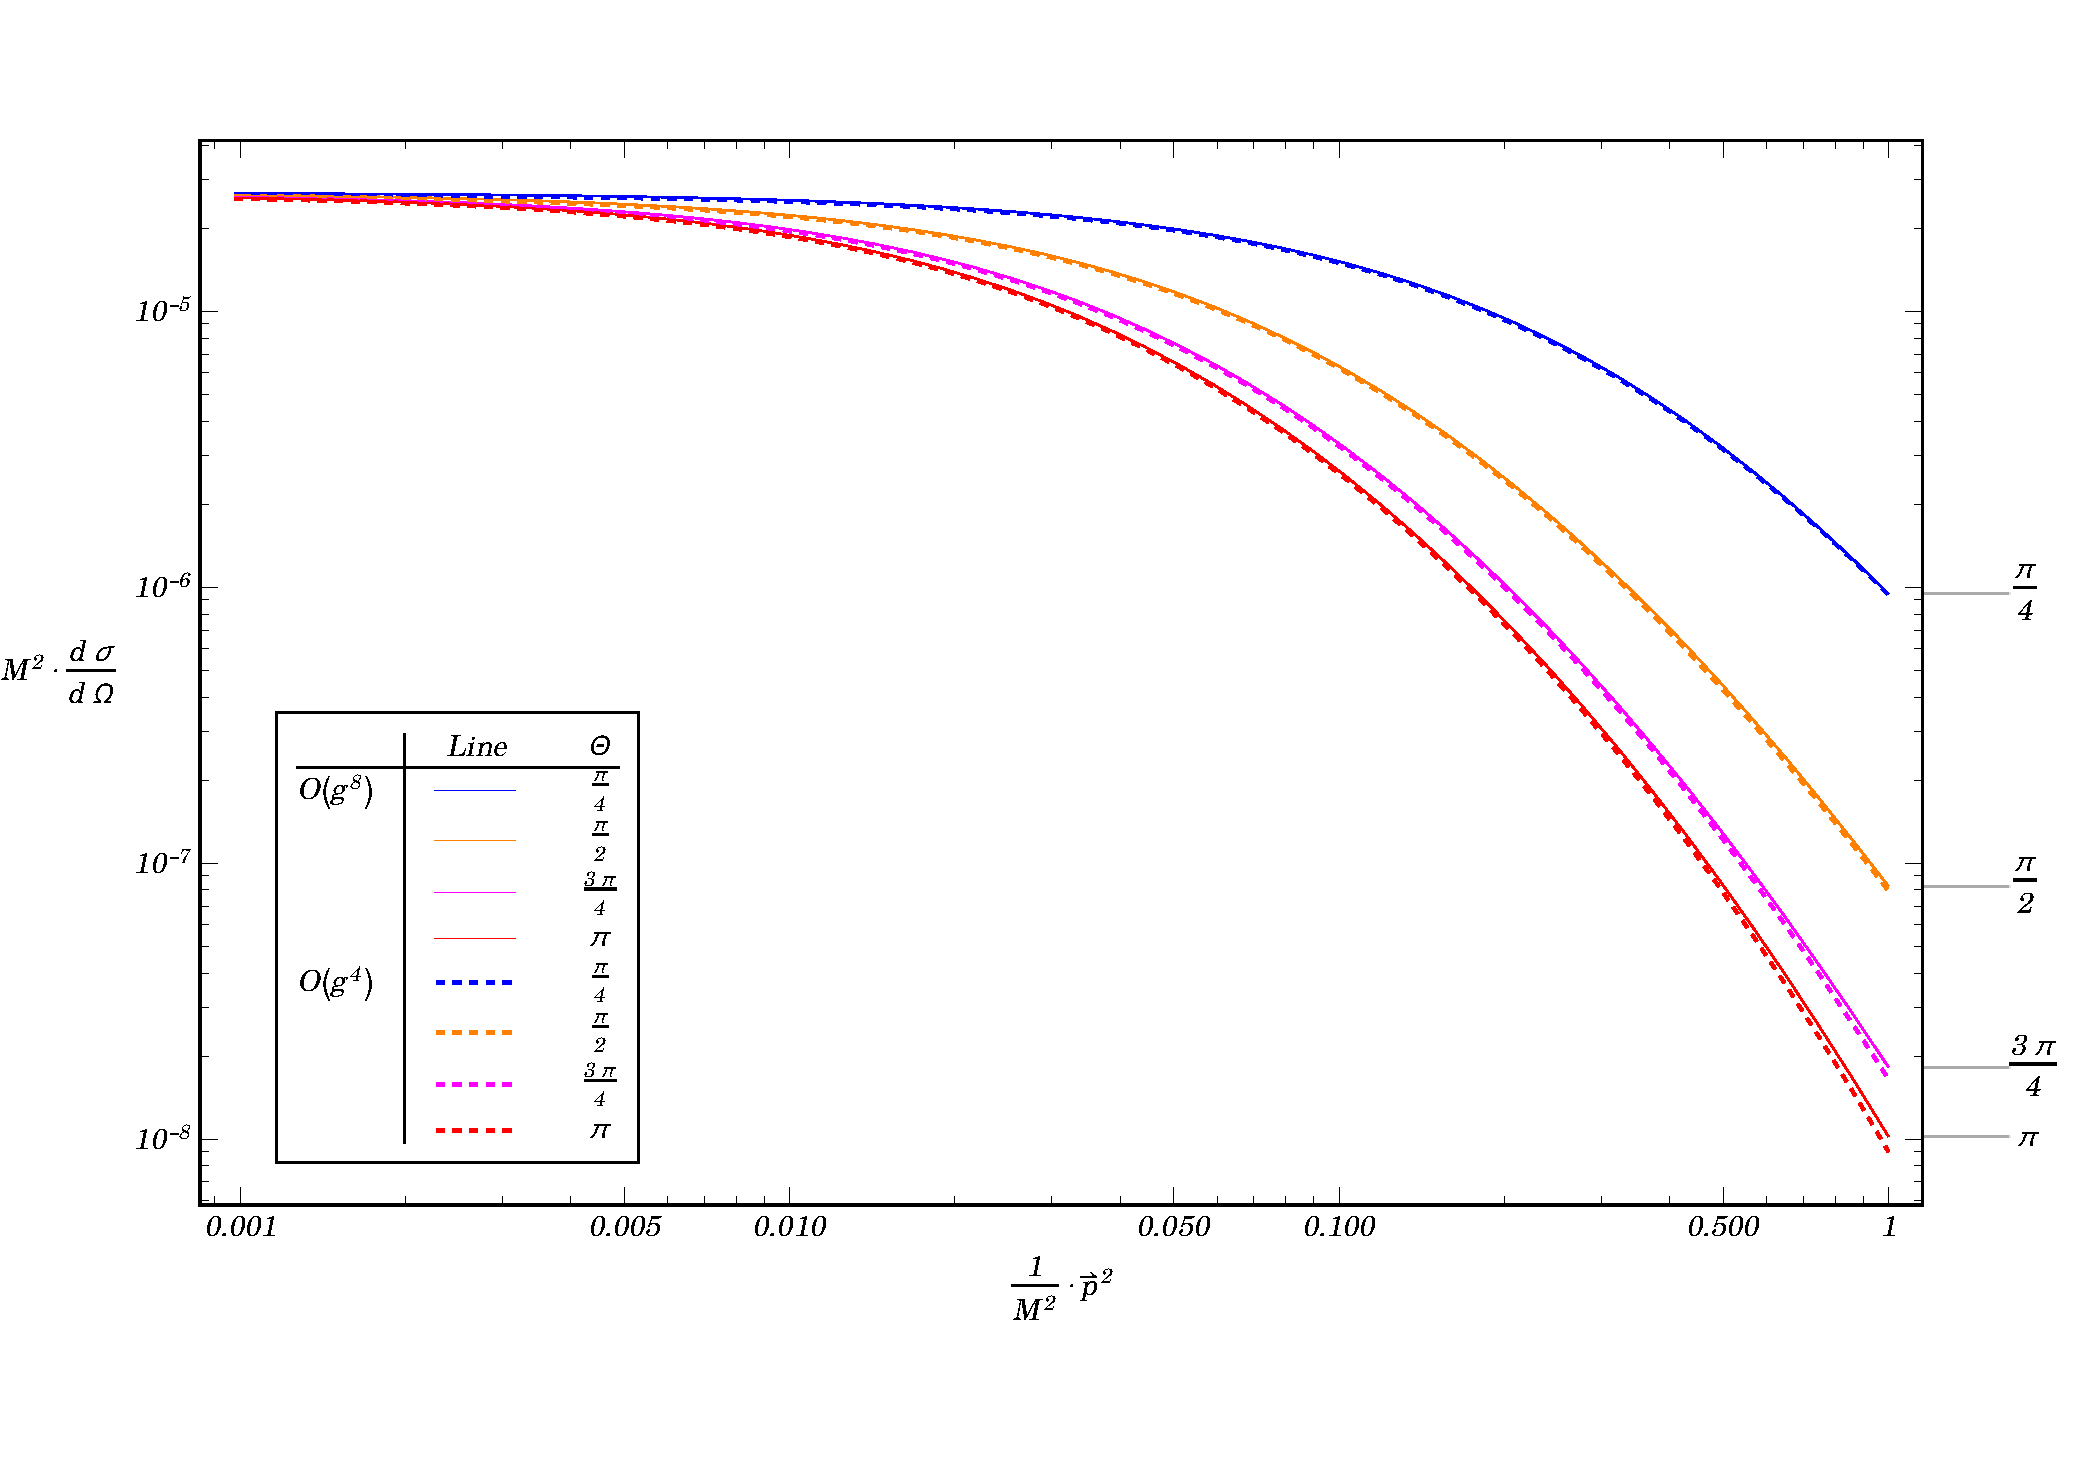
\includegraphics[width=15cm, height=11cm]{StableMeson-LowEnergy}
\caption{Low energy scattering cross section in the stable meson regime with paramters $m = 0.5 M$ and $g = 0.25$. The calculation is performed both at tree-level (dashed) in the cross section and the one-loop level (solid) in perturbation theory at four different fixed values for the scattering angle $\Theta$. The scale is log-log.} 
\label{StabLowEnergy}
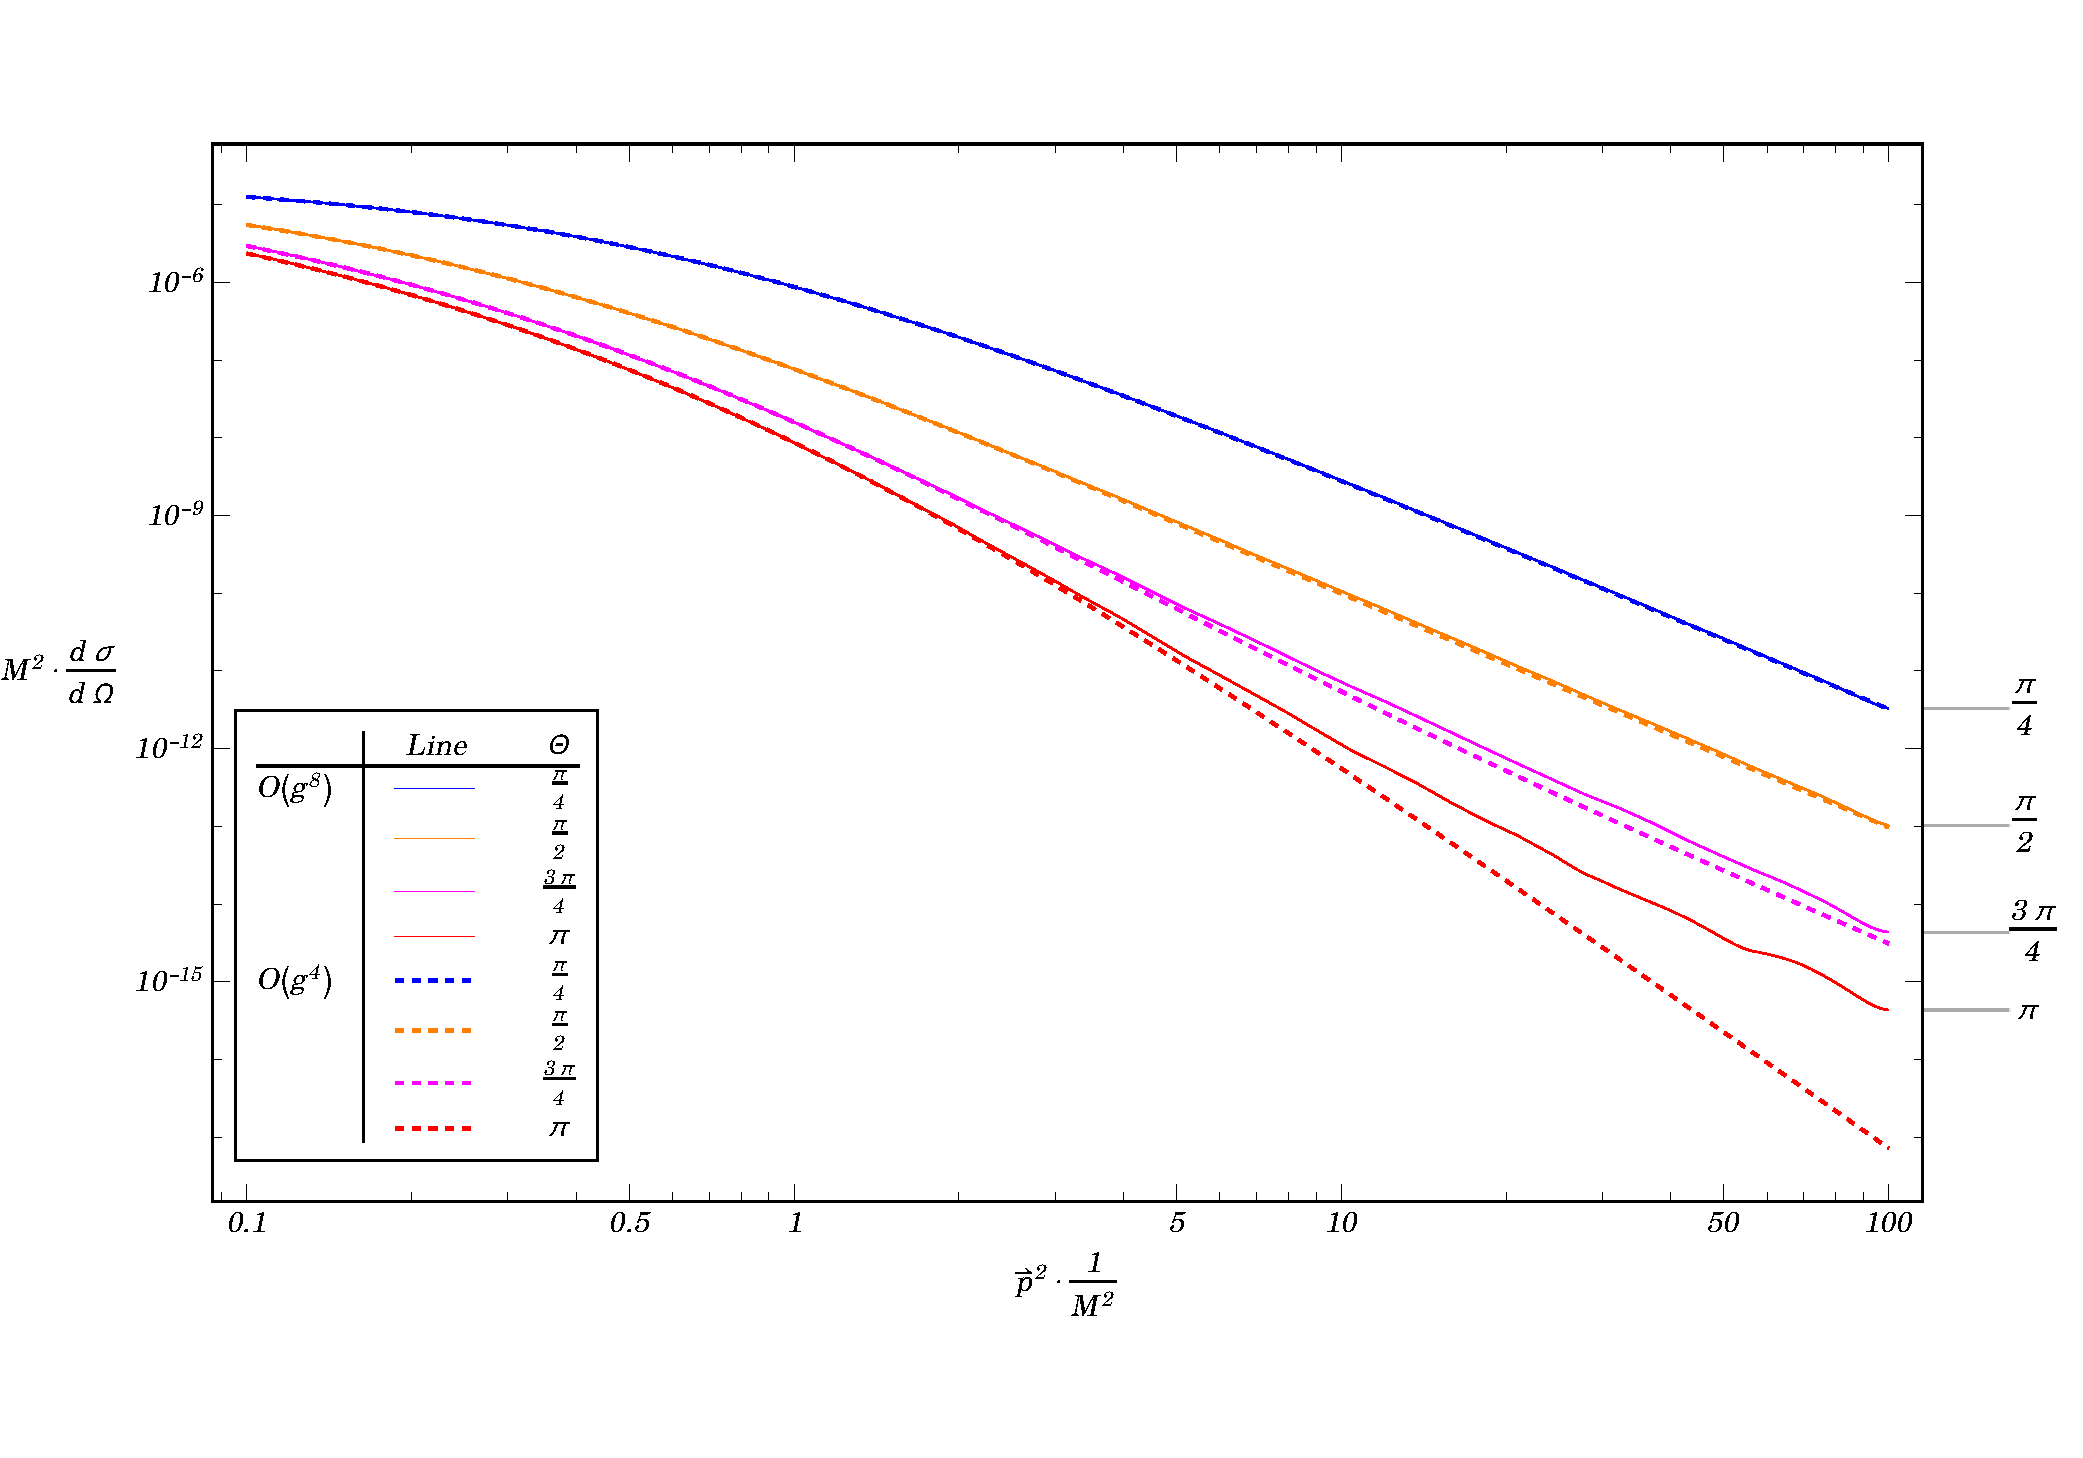
\includegraphics[width=15cm, height=11cm]{StableMeson-HighEnergy}
\caption{High energy scattering cross section in the stable meson regime with paramters $m = 0.5 M$ and $g = 0.25$. The calculation is performed both at tree-level (dashed) in the cross section and the one-loop level (solid) in perturbation theory at four different fixed values for the scattering angle $\Theta$. The scale is log-log.} 
\label{StabHighEnergy}
\end{center}
\end{figure} 


\begin{figure}
\begin{center}
\vspace*{-2cm}
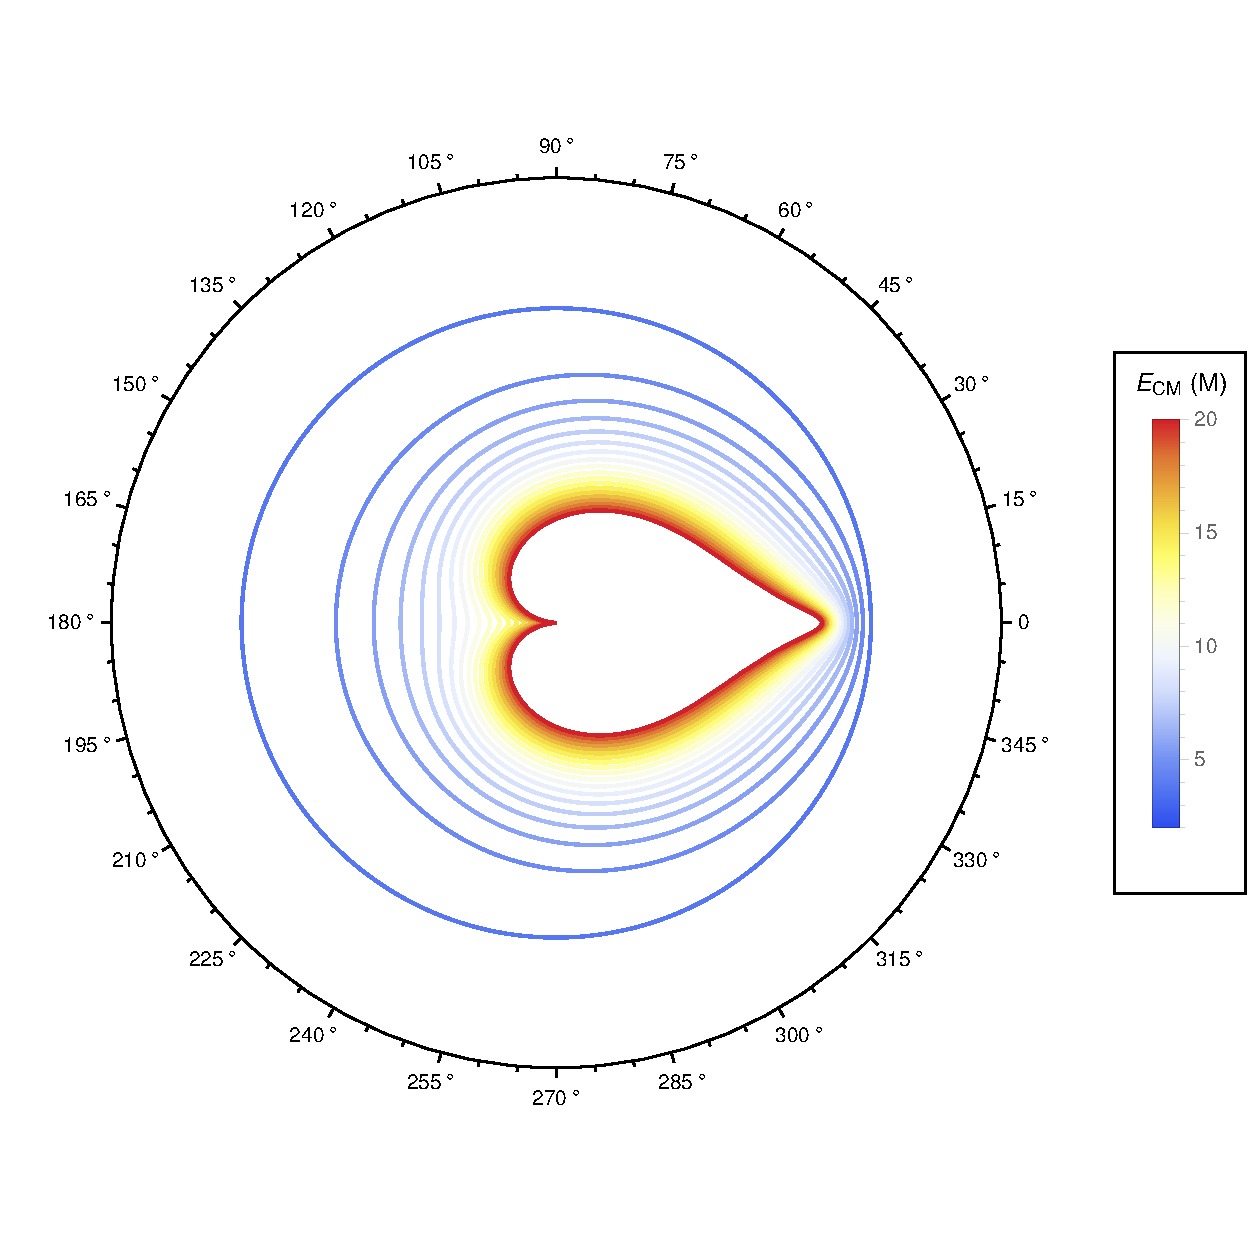
\includegraphics[width=14cm, height=14cm]{StableMeson-LowEnergy-Polar}
\caption{Angluar dependence of the scattering cross section in the stable meson regeme for $m = 0.5 M$. Scattering cross sections are plotted on a log scale. Total scattering energy is expressed in multiples of the $\psi$ rest mass.} 
\label{stable-angular}
\end{center}
\end{figure}

\subsubsection{Scattering in the Unstable Reasonant Regime: $m > 2 M$}
When the meson becomes unstable, two new phenomena appear. When the total scattering energy equals the mass energy of the meson, a resonance in the scattering amplitude forms due to the creation of a semistable meson as an intermediate product in the process $\psi \bar{\psi} \to \phi \to \psi \bar{\psi}$. This resonance only appears in $s$-channel diagrams because it relies on the possibility of $\psi-\bar{\psi}$ annhilation. Along with resonances, anti-resonances appear in the scattering amplitude only in the regime $m > 2 M$. At an anti-resonance, the scattering amplitude drops nearly (at tree-level exactly) to zero due to destructive interference between the $s$ and $t$-channel amplitudes. At a fixed energy, the destructive interference only occurs for a fixed scattering angle $\Theta$. Figure \ref{unstable-angular}. shows how the position of the anti-resonance shifts towards back-scattering in the high energy limit. For exact back-scattering or forward-scattering, no anti-resonance occurs. However, at any other fixed scattering angle there is a particular total energy at which the destructive interference occurs in that direction.\bigskip\\
The imaginary part of the dressed propagator for $\phi$ smooths both the resonances and anti-resonances such that the scattering amplitude does not have poles or zeros for physical scattering energies. Furthermore, the contribution of box diagrams shifts the location of the destructive interference and somewhat softens the cusp (see figure \ref{AntiResonance}.) The quadratic nature of these anti-resonances due to destructive interference can be seen when the amplitude is viewed on a linear scale as in figure \ref{NoLogAntiResonance}.    


\begin{figure}
\begin{center}
\vspace*{-2cm}
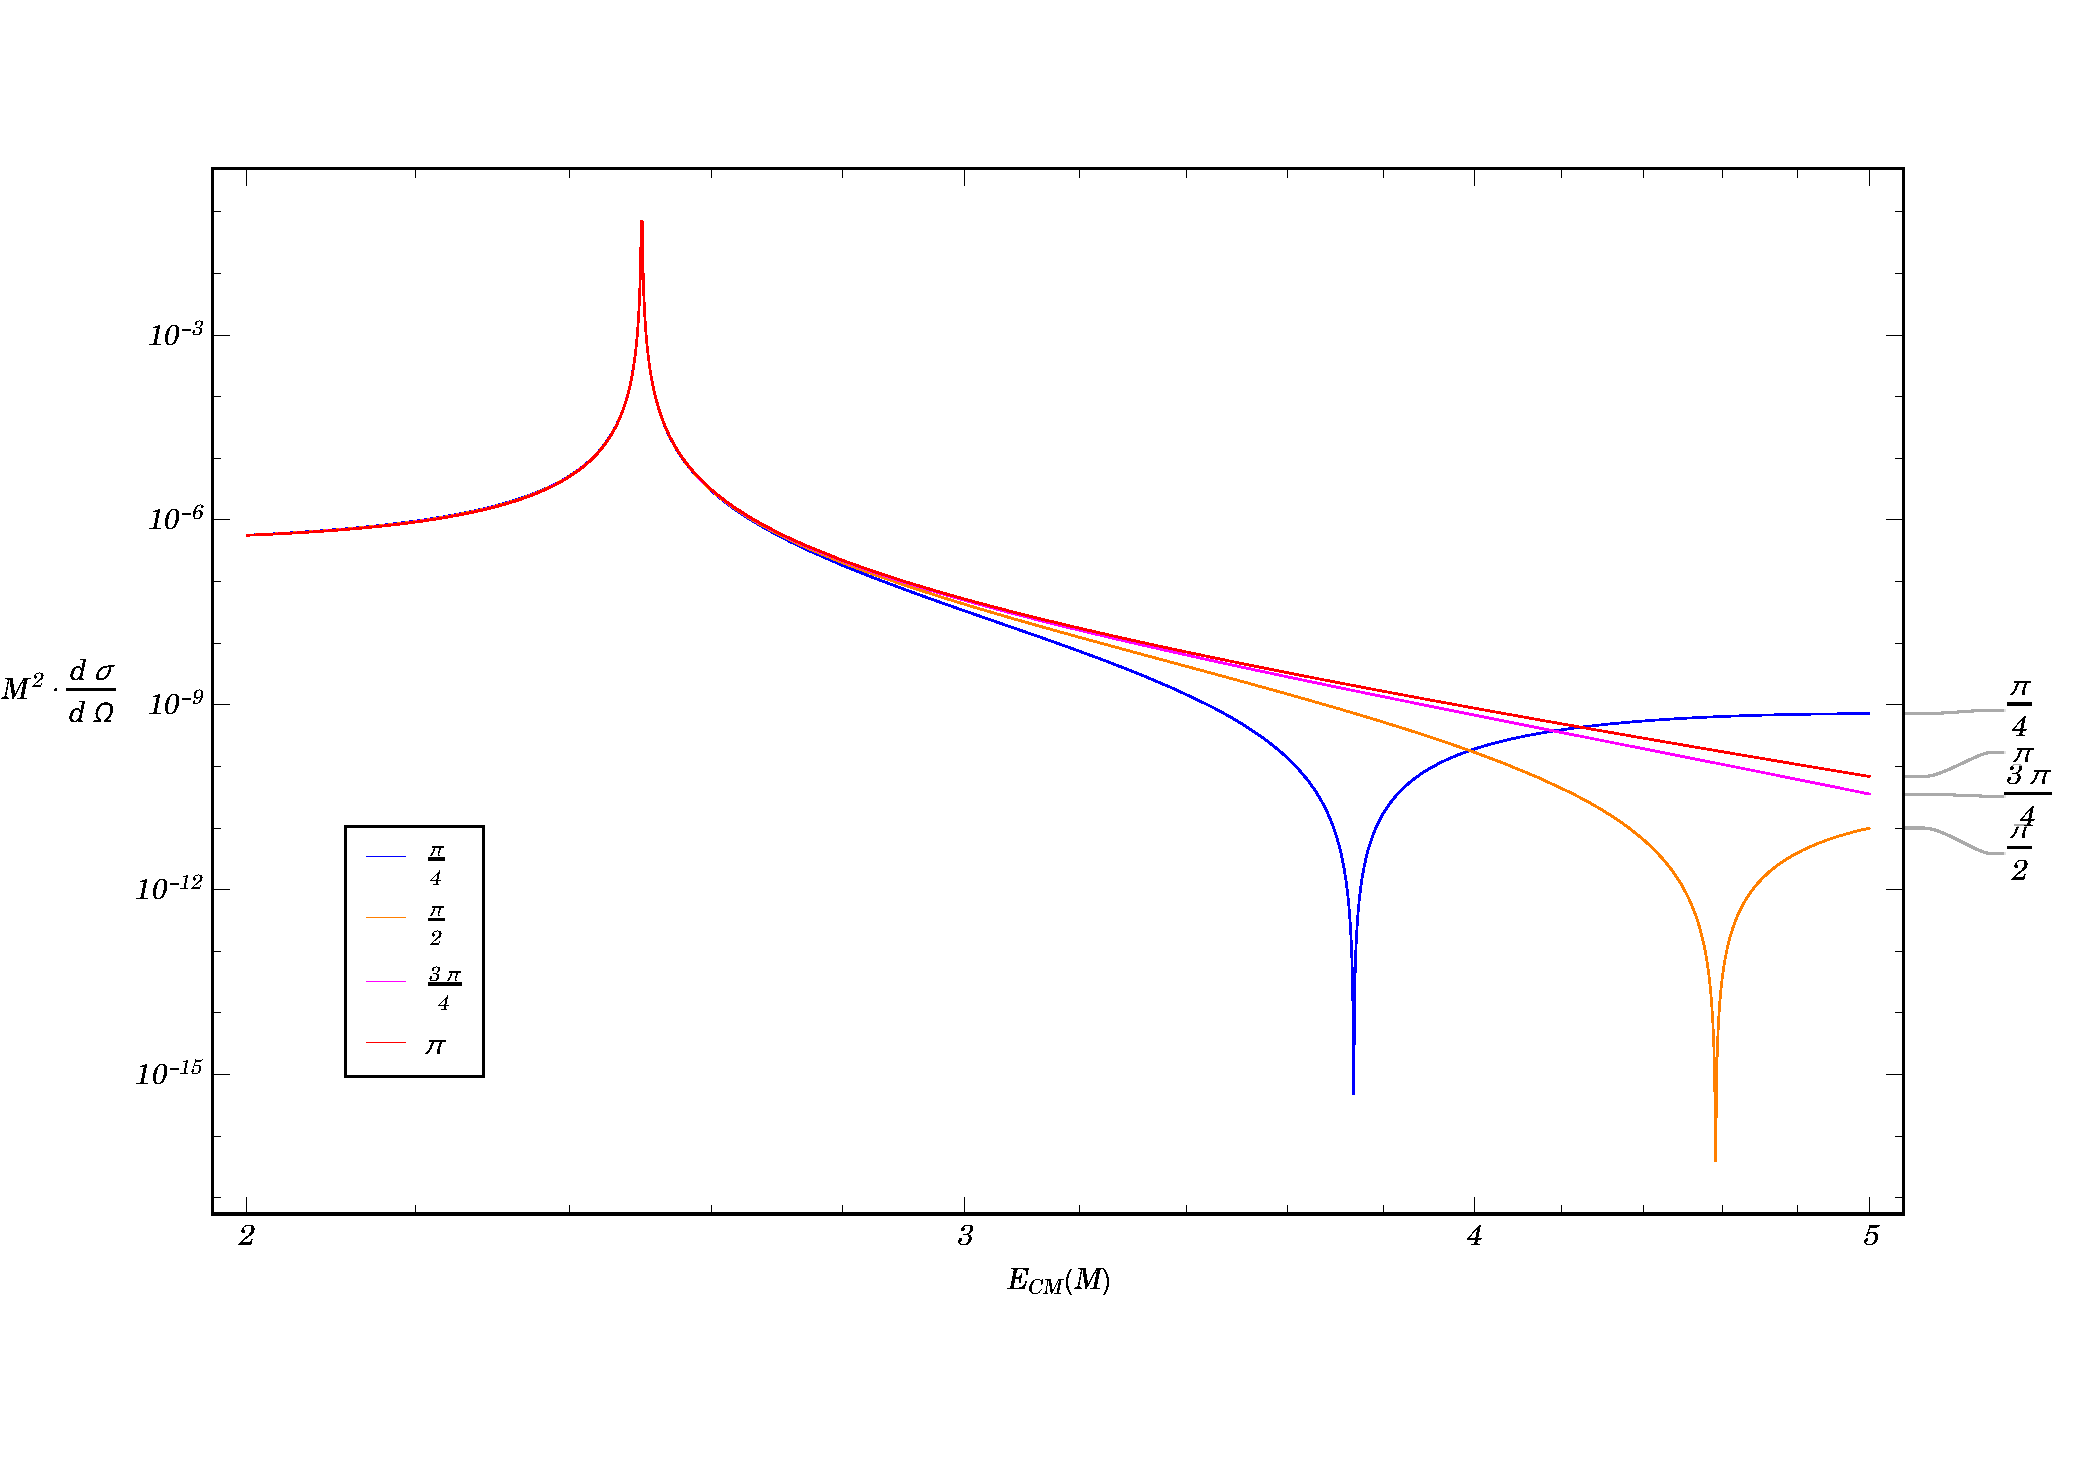
\includegraphics[width=15cm, height=11cm]{UnStableMeson-LowEnergy}
\caption{Low energy scattering cross section in the unstable meson regime with paramters $m = 2.5 M$ and $g = 0.25$. The calculation is performed both at tree-level (dashed) in the cross section and the one-loop level (solid) in perturbation theory at four different fixed values for the scattering angle $\Theta$. The scale is log-log.} 
\label{UnStabLowEnergy}
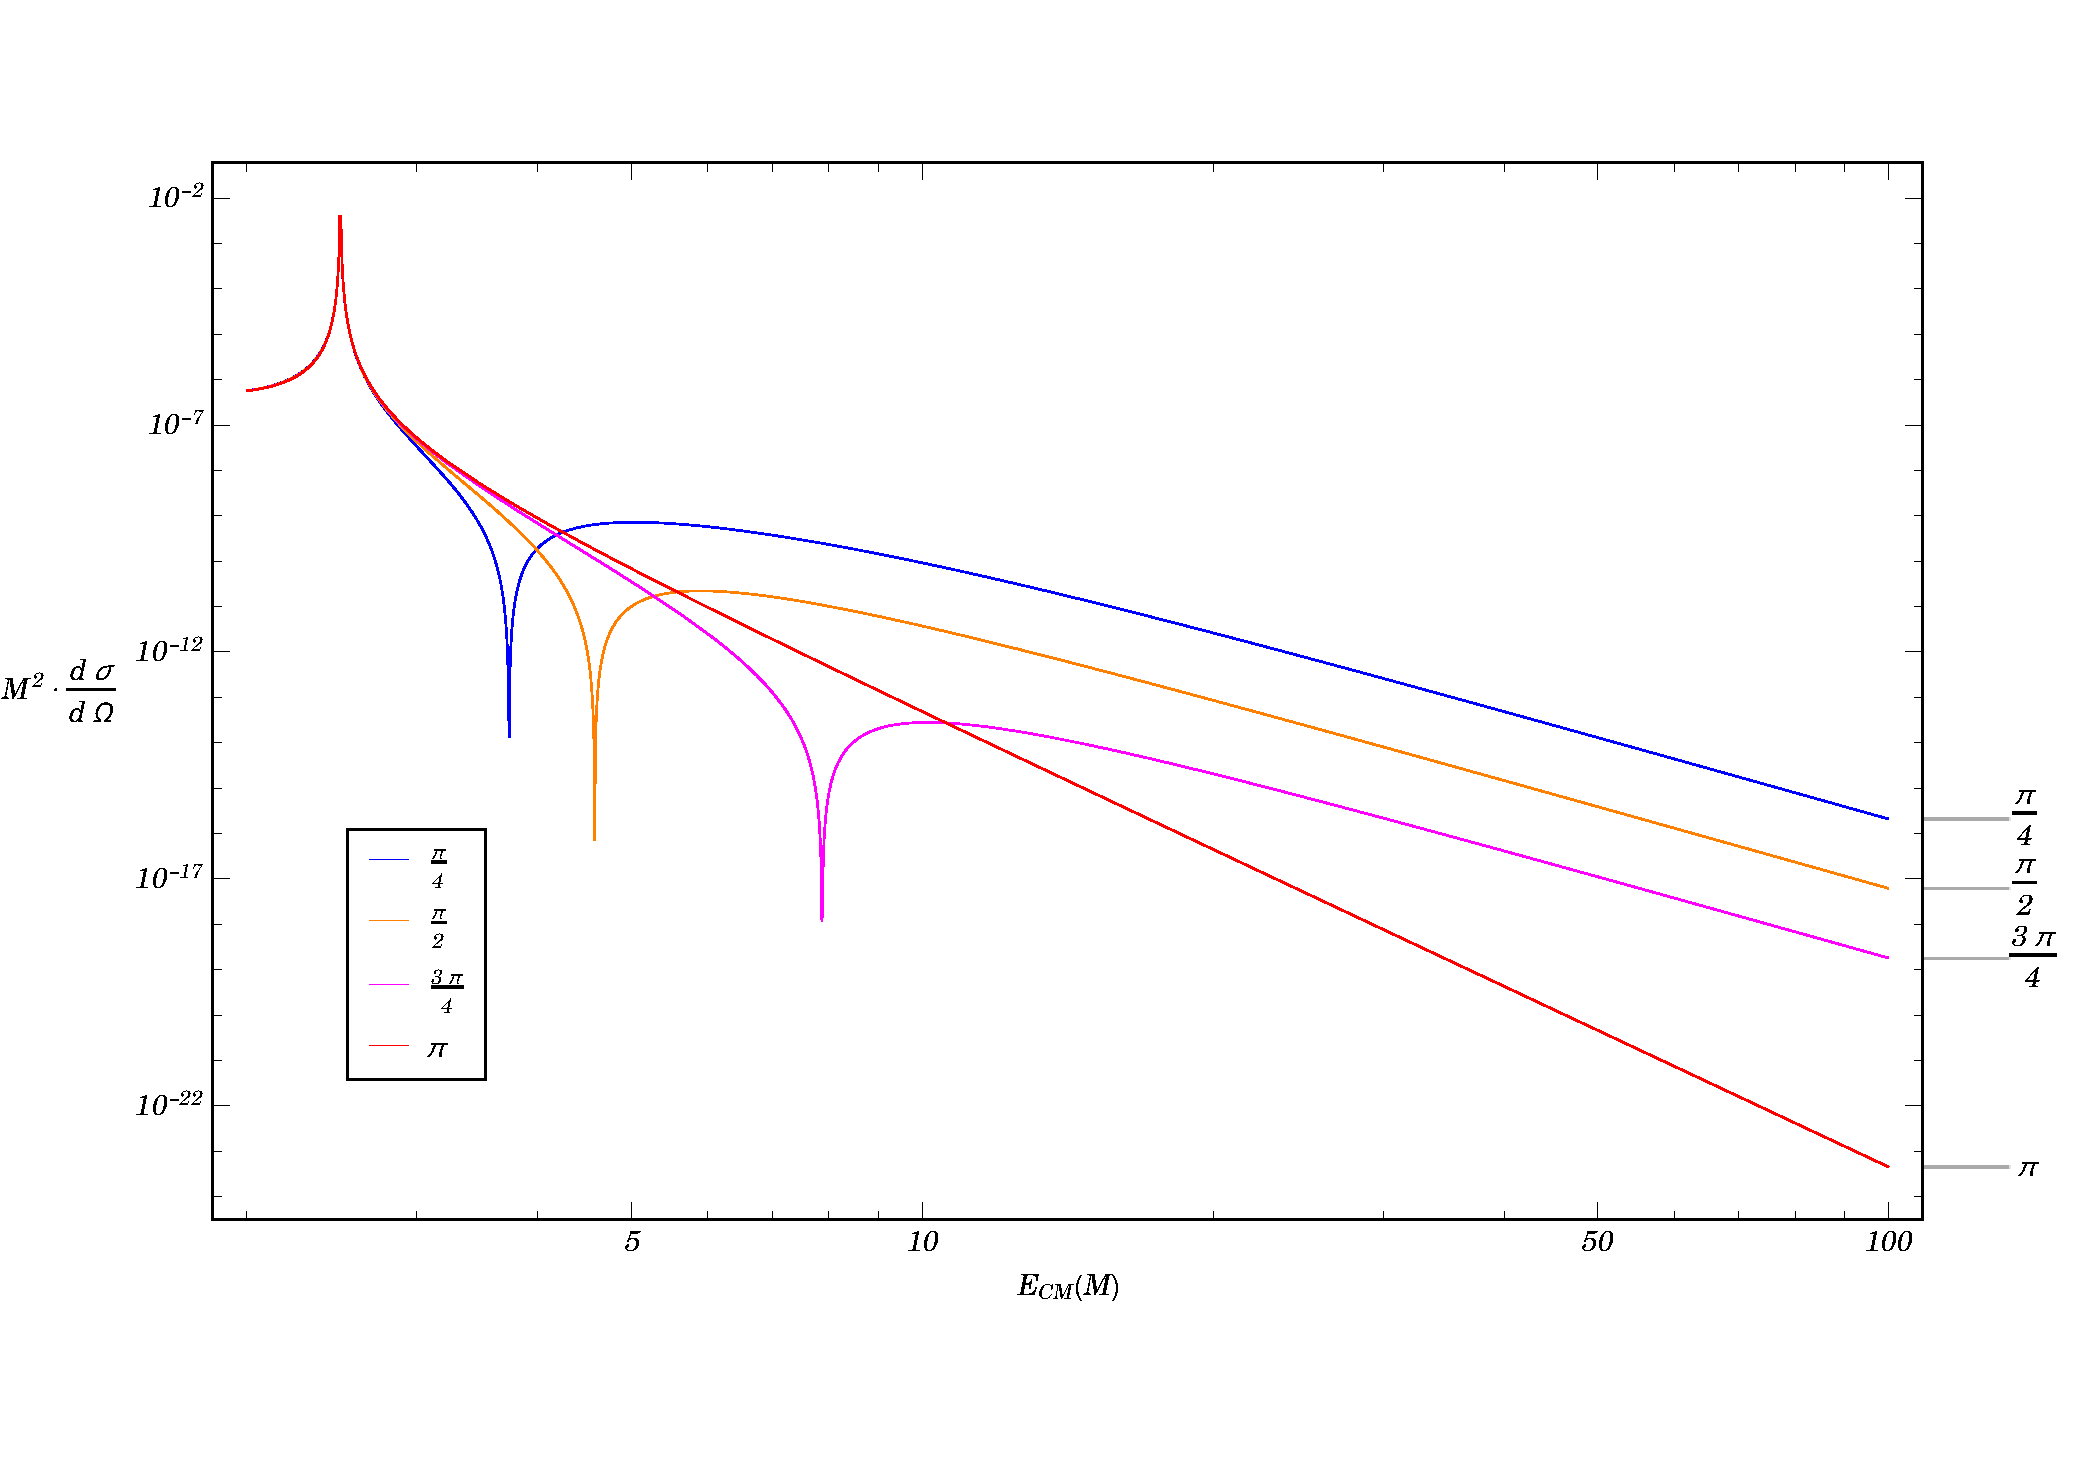
\includegraphics[width=15cm, height=11cm]{UnStableMeson-HighEnergy}
\caption{High energy scattering cross section in the unstable meson regime with paramters $m = 2.5 M$ and $g = 0.25$. The calculation is performed both at tree-level (dashed) in the cross section and the one-loop level (solid) in perturbation theory at four different fixed values for the scattering angle $\Theta$. The scale is log-log. Energies are expressed im multiples of the $\psi$ particle rest mass.} 
\label{UnStabHighEnergy}
\end{center}
\end{figure} 

\begin{figure}
\begin{center}
\vspace*{-2.5cm}
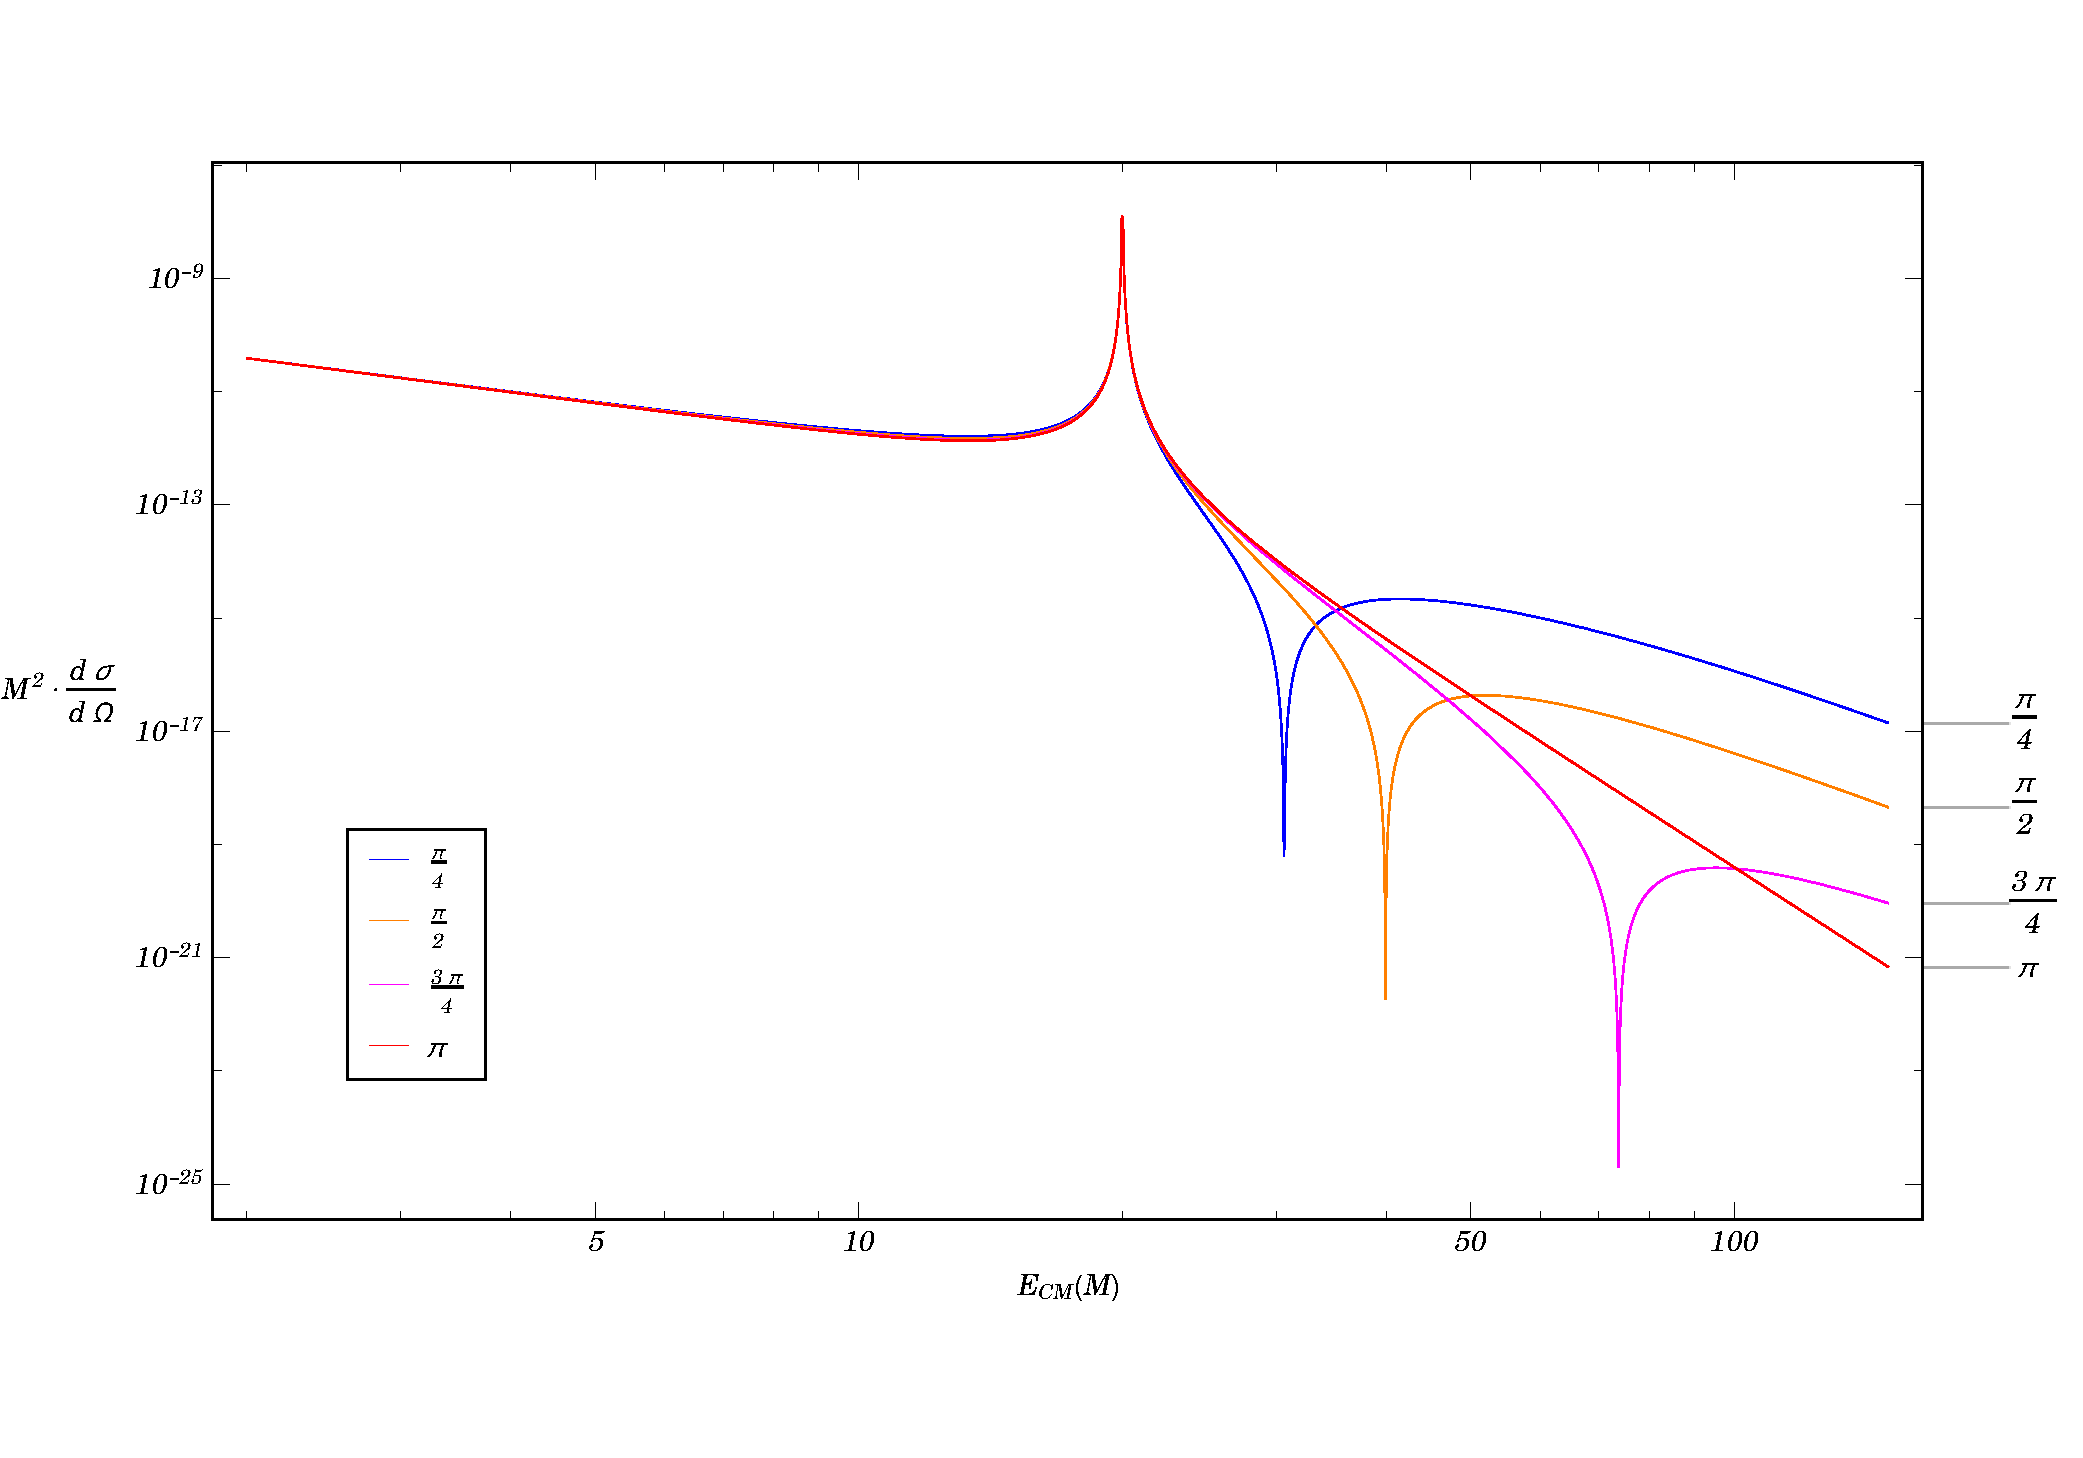
\includegraphics[width=15cm, height=11cm]{HighMass-UnStableMeson-HighEnergy}
\vspace*{-0.5cm}
\caption{Low energy scattering cross section for heavy mesons with parameters $m = 20 M$ and $g = 0.25$. The calculation is performed both at tree-level (dashed) in the cross section and the one-loop level (solid) in perturbation theory at four different fixed values for the scattering angle $\Theta$. The scale is log-log. Energies are expressed im multiples of the $\psi$ particle rest mass.} 
\label{HighMassUnStabHighEnergy}
\vspace*{-0.5cm}
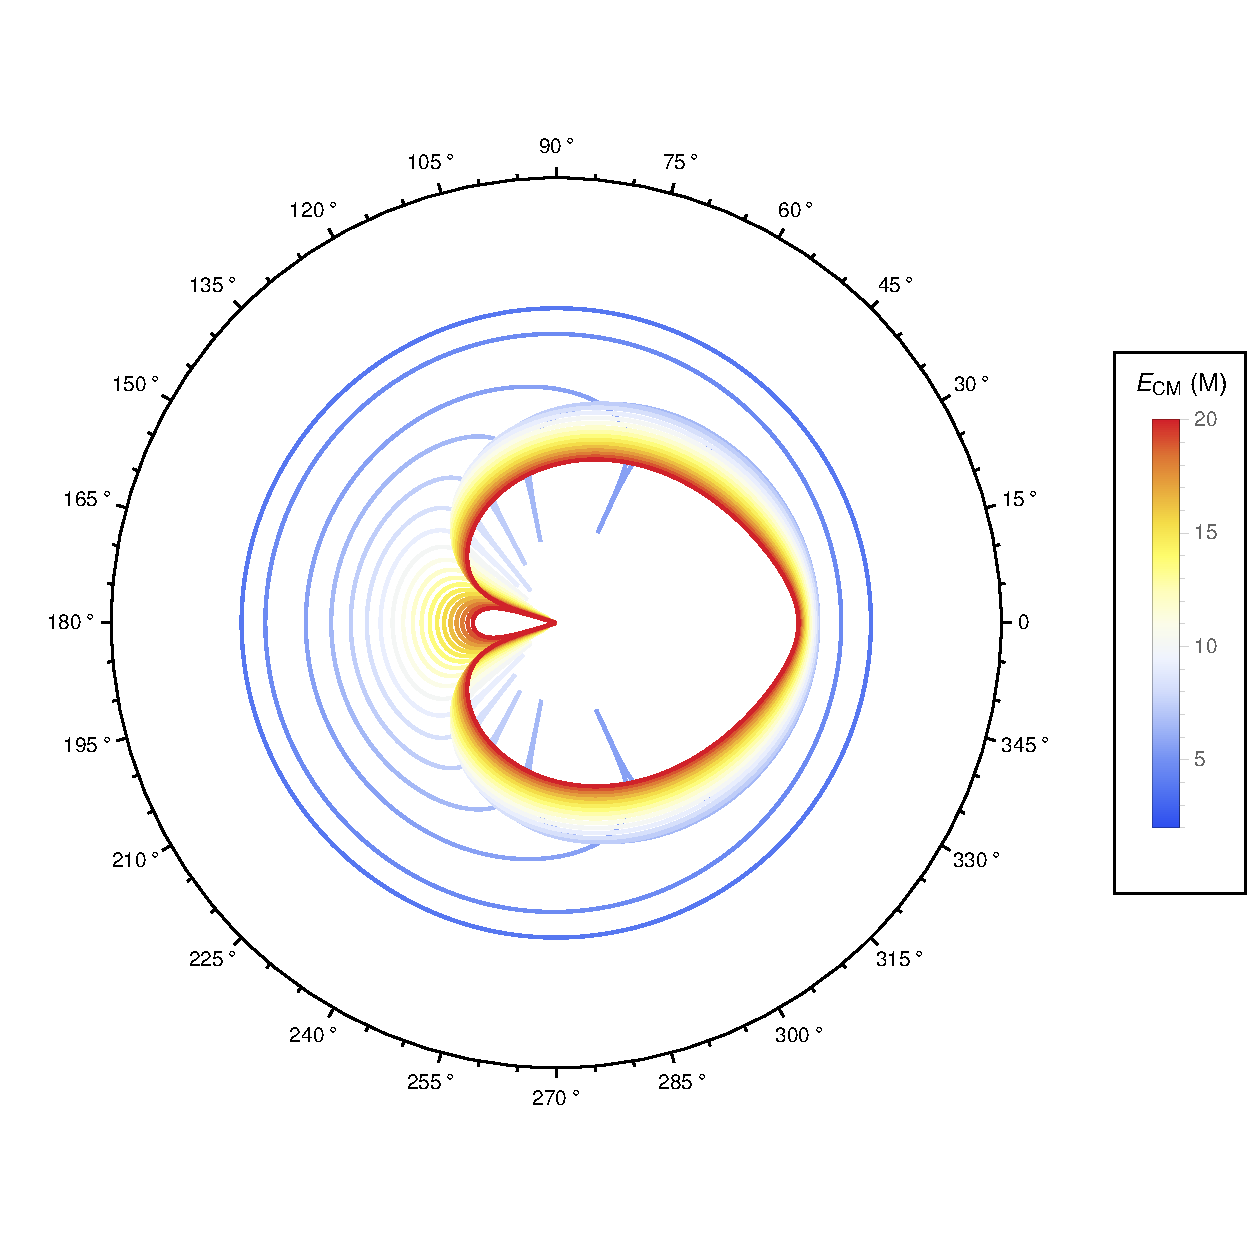
\includegraphics[width=14cm, height=14cm]{UnStableMeson-LowEnergy-Polar}
\vspace*{-1cm}
\caption{Angluar dependence of the scattering cross section in the unstable meson regeme with $m = 2.5 M$. Scattering cross sections are plotted on a log scale. Total scattering energy is expressed in multiples of the $\psi$ rest mass.} 
\label{unstable-angular}
\end{center}
\end{figure} 


\begin{figure}
\begin{center}
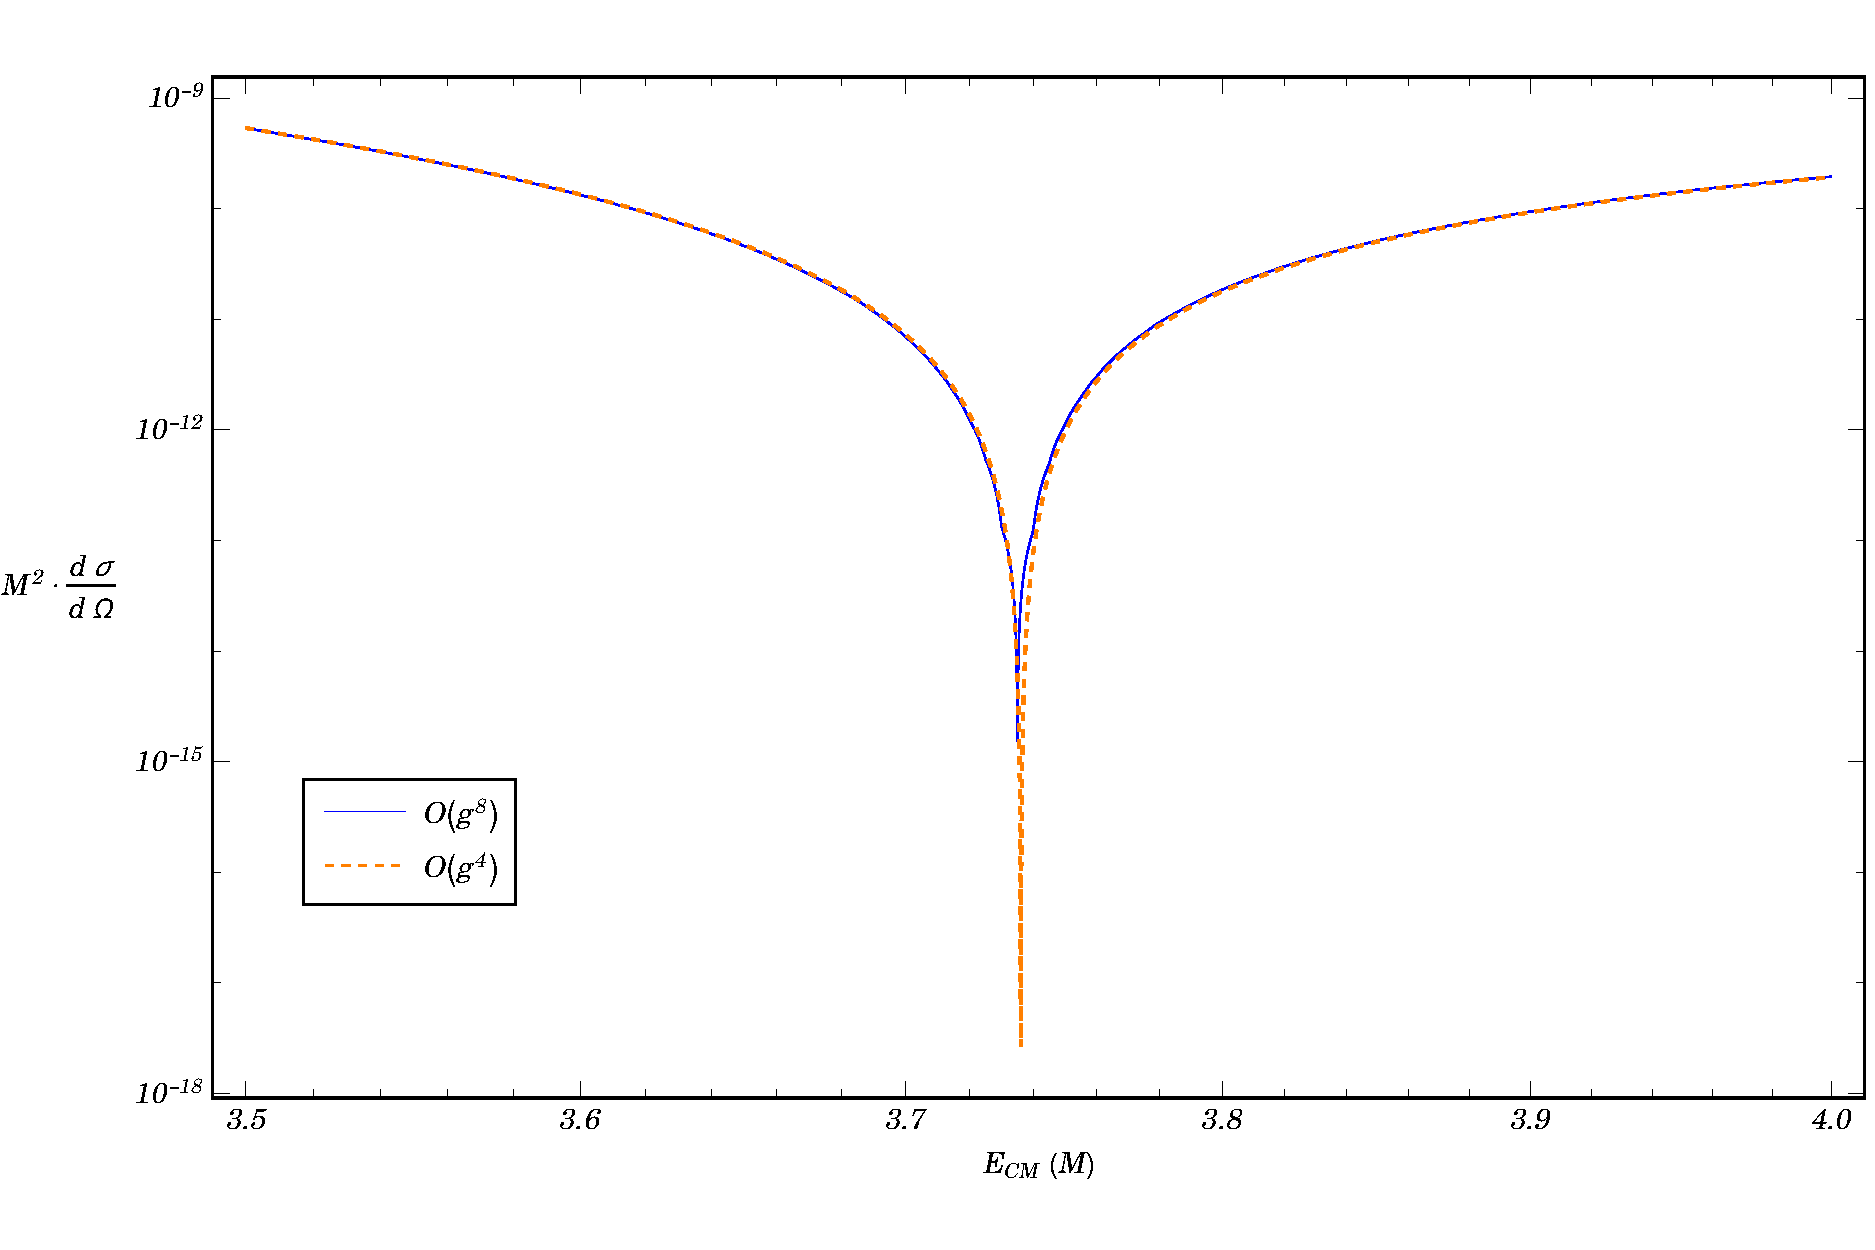
\includegraphics[width=15cm, height=10cm]{AntiResonance}
\caption{Closeup of destructive interference of the cross section at a fixed scattering angle in the unstable meson regeme with $m = 2.5 M$ and $\Theta = \frac{\pi}{4}$. Scattering cross sections are plotted on a log scale. Total scattering energy is expressed in multiples of the $\psi$ rest mass.} 
\label{AntiResonance}
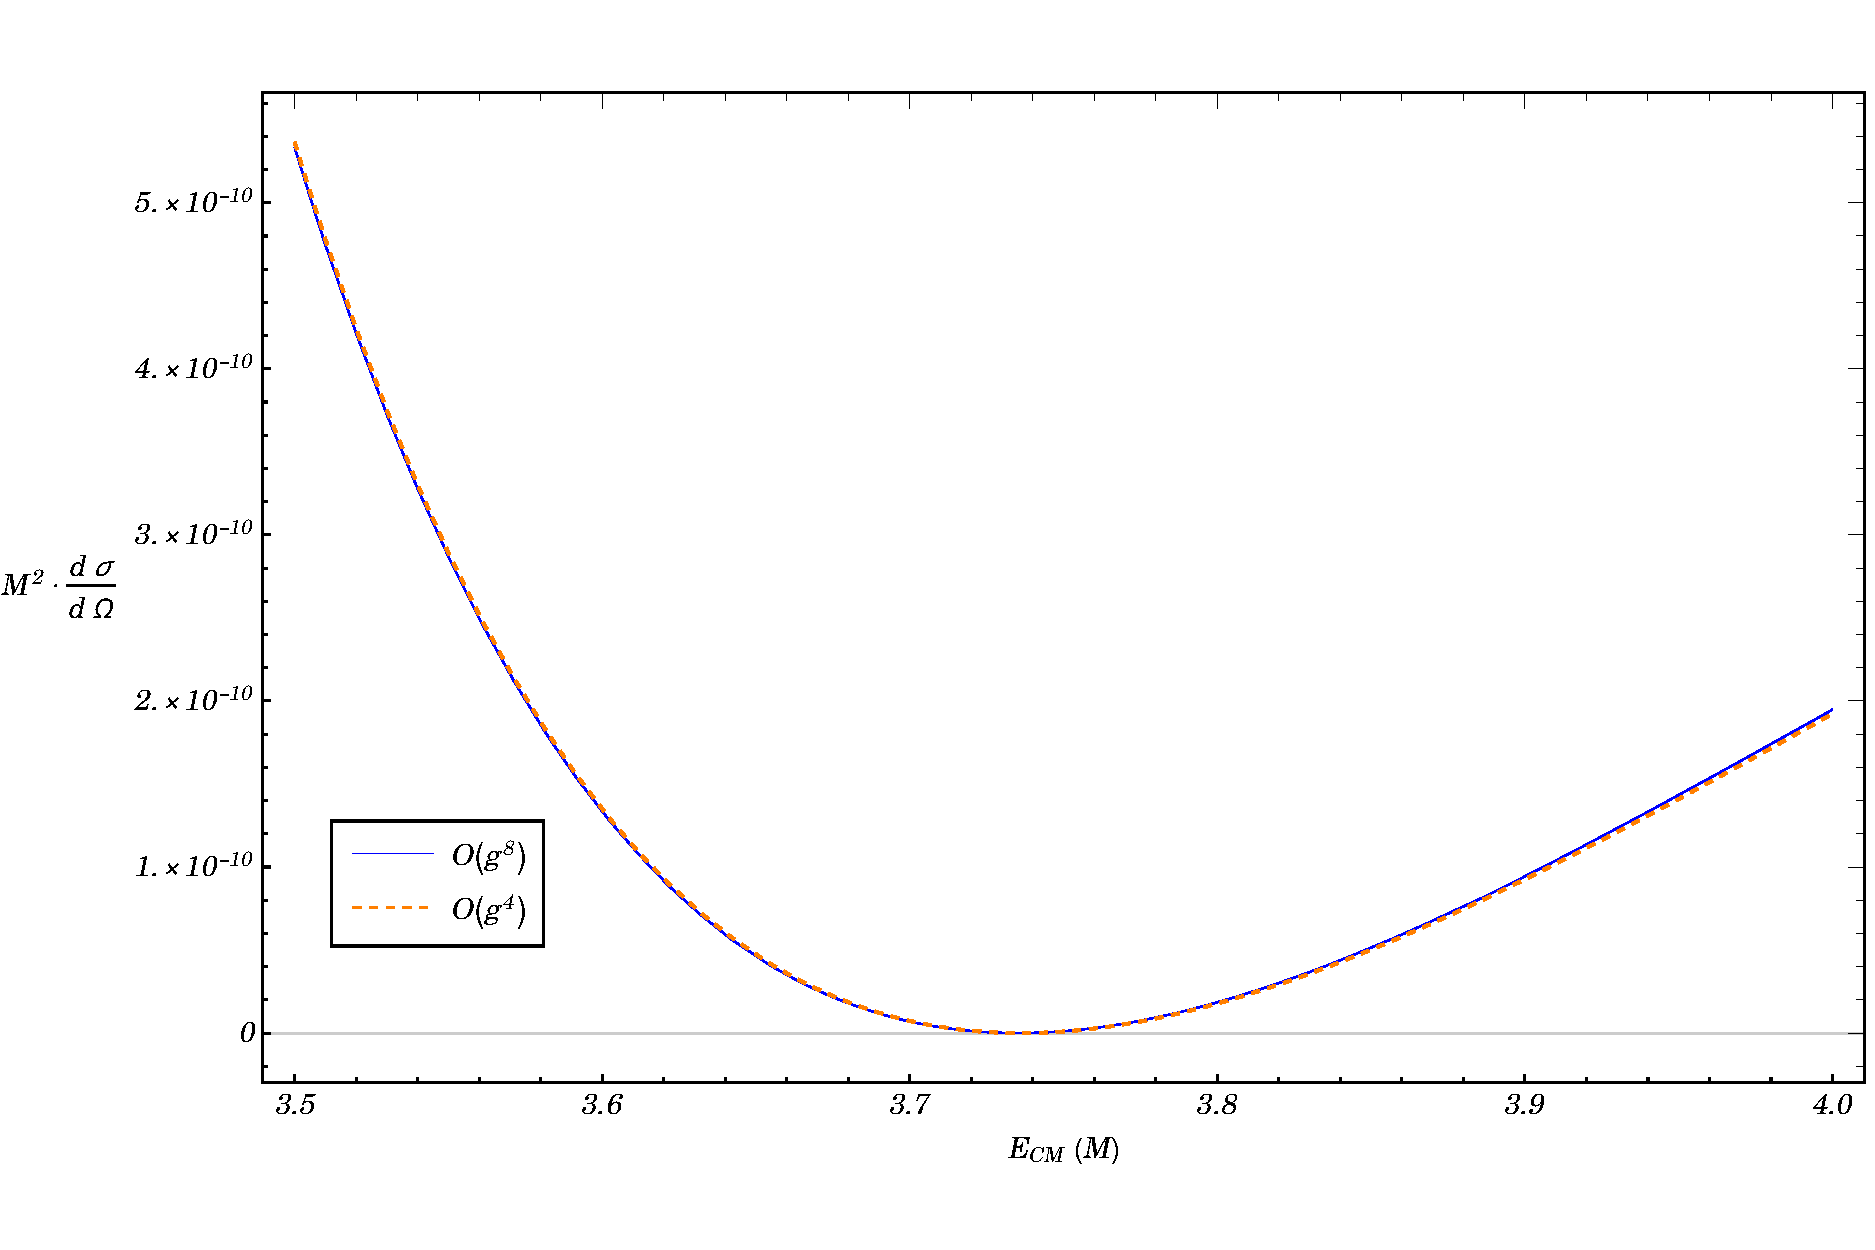
\includegraphics[width=15cm, height=10cm]{NoLogAntiResonance}
\caption{Closeup of destructive interference of the cross section at a fixed scattering angle in the unstable meson regeme with $m = 2.5 M$ and $\Theta = \frac{\pi}{4}$. Scattering cross sections are plotted on a linear scale. Total scattering energy is expressed in multiples of the $\psi$ rest mass.} 
\label{NoLogAntiResonance}
\end{center}
\end{figure}

\subsubsection{Illustration of Scattering Resonance}
Even in the regime in which the meson is unstable, the interaction is weak enough that the meson is quite long-lived and therefore the scattering resonance is extremely sharp. To illustrate the appearence of a Breit-Winger distribution in the scattering applitude due to resonances of unstable particles we employ an toy model of the toy scalar Yukawa theory. To do this, I will set $g = 4 M$ so we are far into the unpertubative regime in which our truncation of the Dyson series is not partucularly well justified. That said, our trucated scattering amplitude is illustrative of resonance peaks in strongly coupled theories with highly unstable particles. In particular, as shown in figure \ref{Ill}. the full meson propagator has an imaginary part due to allowed decay channels which reduces the shaprness of the resonant peak. Similarly, the full propagator has the effect of shifting the energy (at a fixed scattering angle) at which destructive intereference between the $s$ and $t$-channels occurs. Furthermore, the imaginary part of the propagator also obstructs the scattering amplitude from reaching zero at the point of destructive interference.     
\begin{figure}
\begin{center}
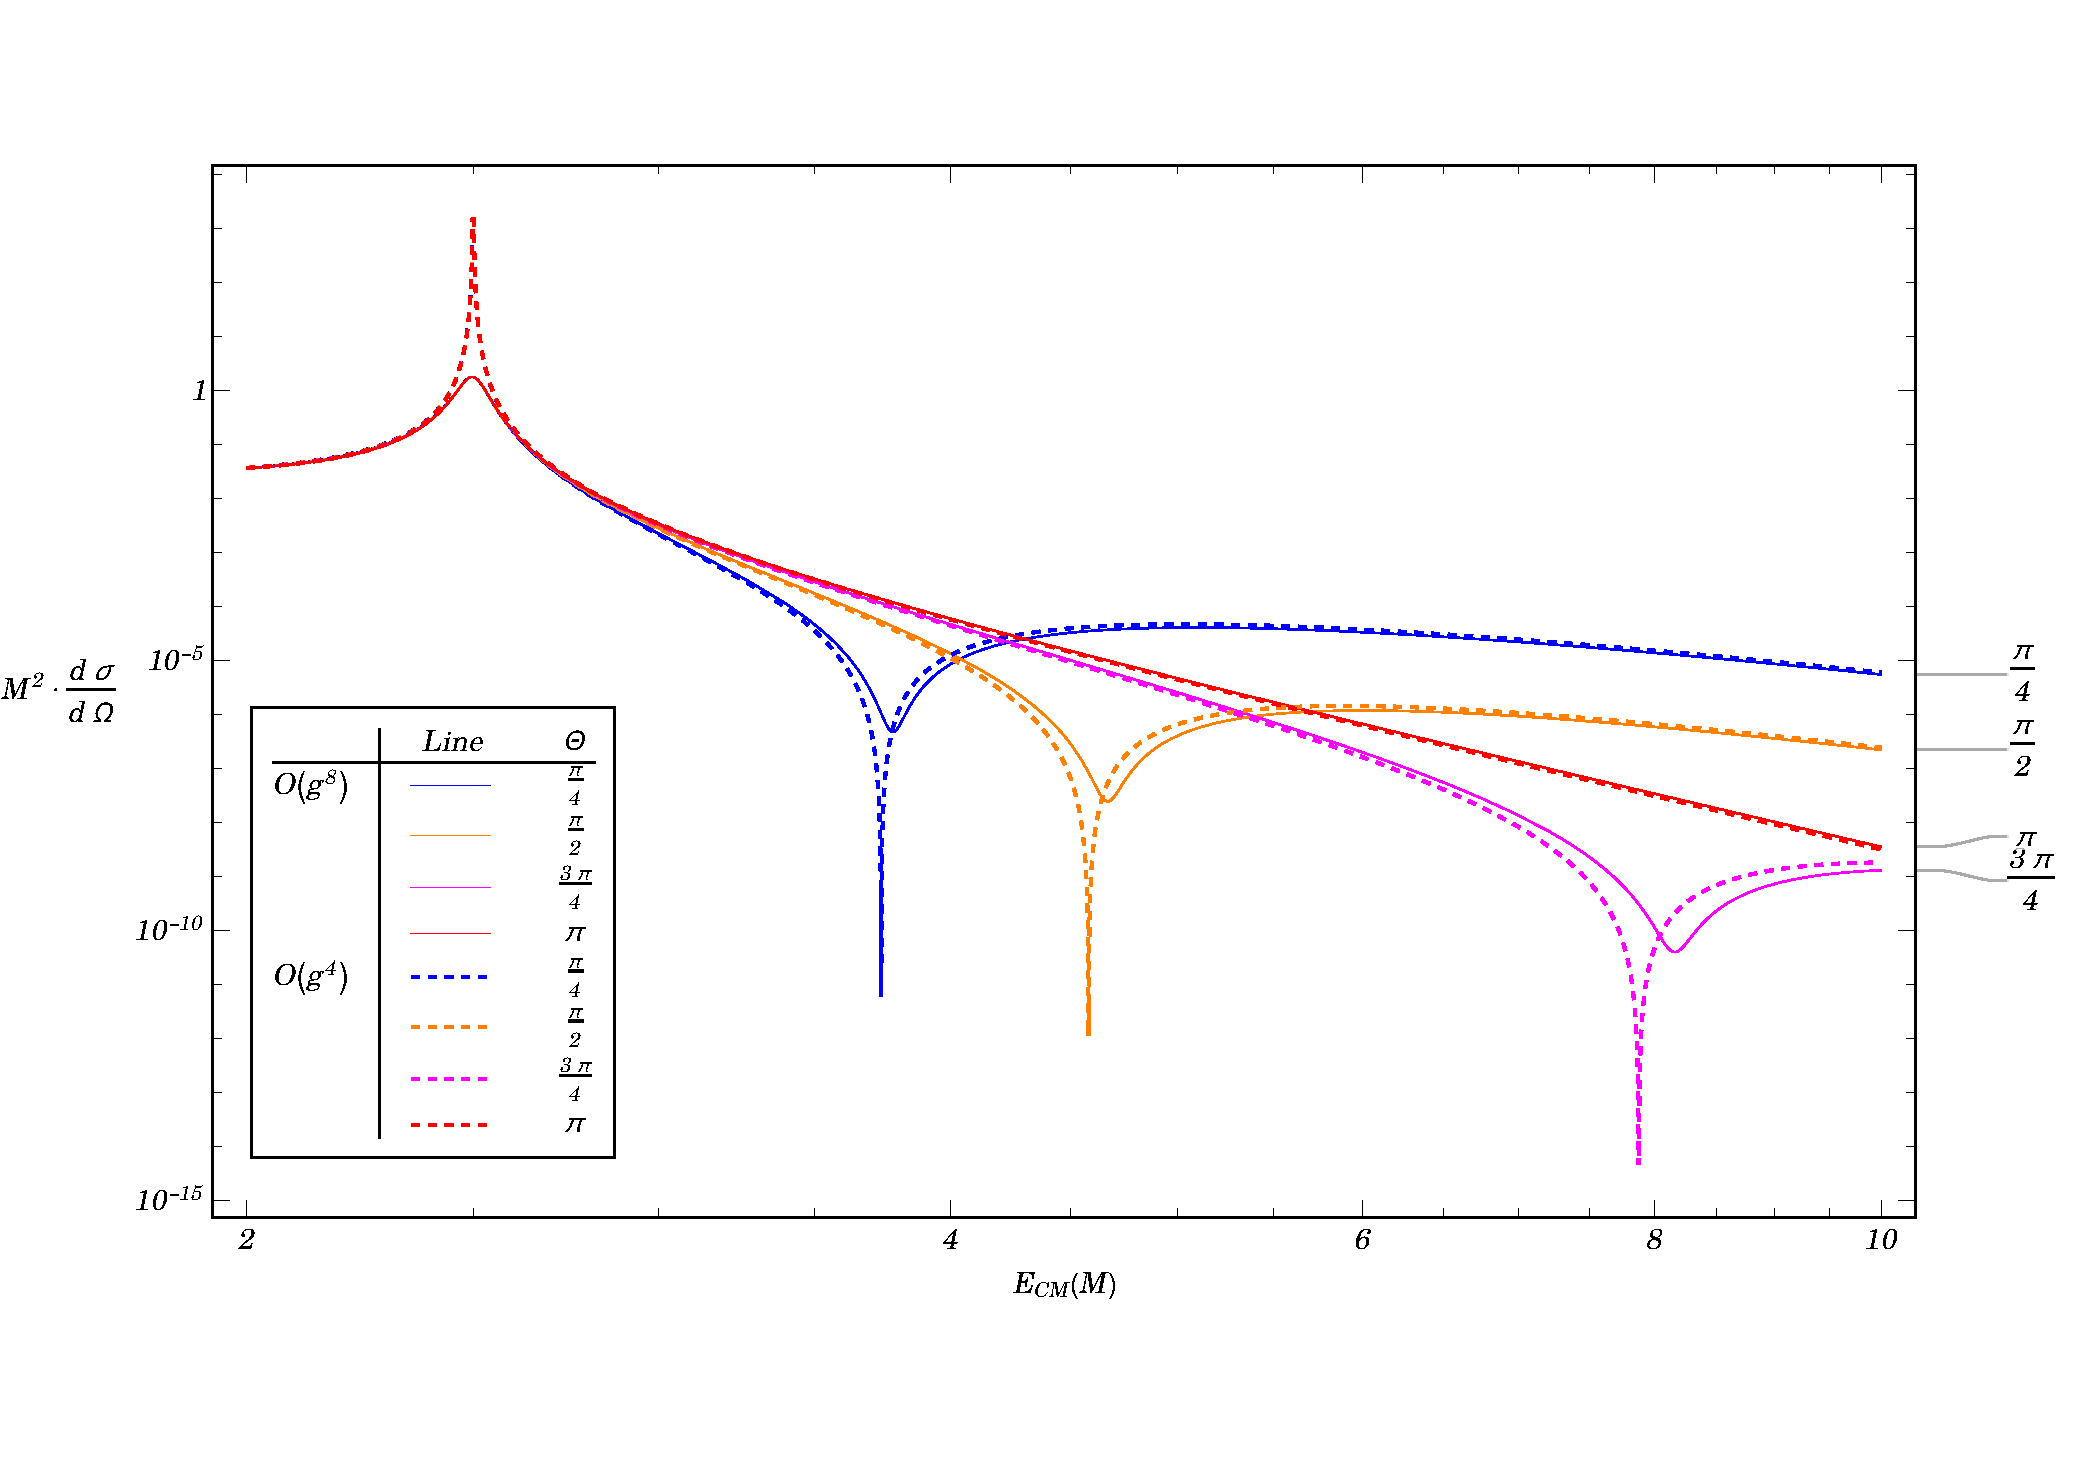
\includegraphics[width=15cm, height=11cm]{UnStableMeson-Illustration}
\caption{Scattering cross section versus total scattering energy for the strongly coupled theory ($g = 4 M$) at both tree-level and the one-loop level in the unstable meson regime $m = 2.5 M$. Curves show the scattering amplitude at a fixed scattering angle. Solid lines are the full one-loop calculation such that the cross section is exact to $O(g^8)$. Dashed lines are the tree-level result which is order $g^4$ in the scattering amplitude. The scale is log-log. Energies are expressed im multiples of the $\psi$ particle rest mass.} 
\label{Ill}
\end{center}
\end{figure}

\begin{figure}
\begin{center}
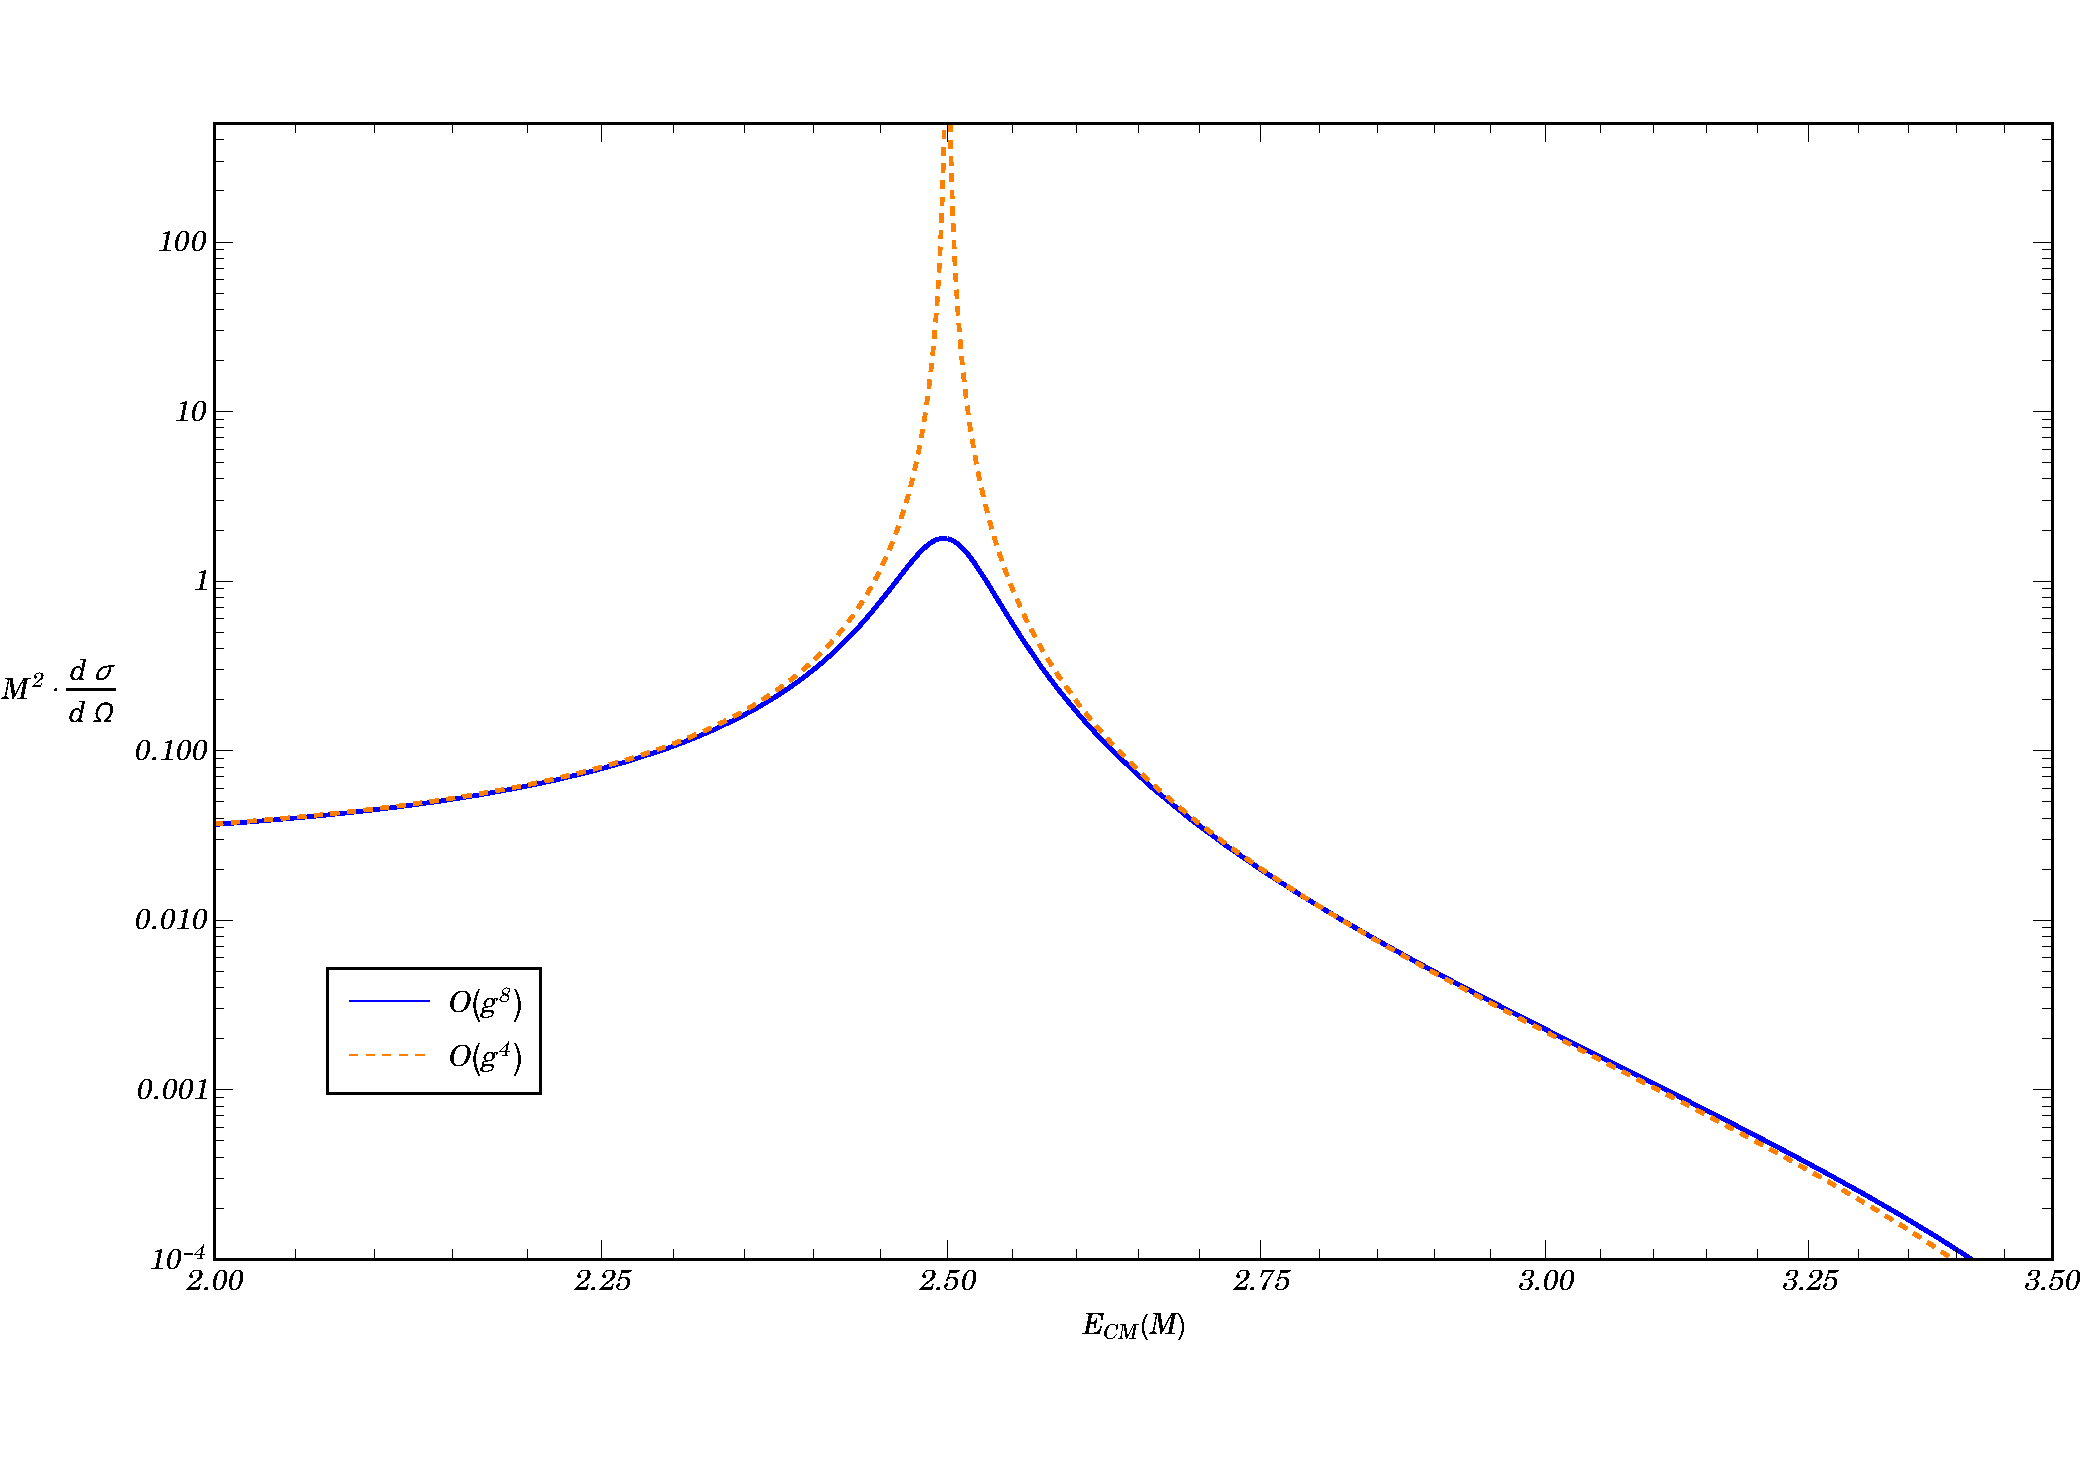
\includegraphics[width=15cm, height=11cm]{Resonance-Illustration}
\caption{Closeup of scattering cross section resonance due to (nearly) on-shell virtual meson in the strongly interacting ($g = 4 M$) unstable meson regeme with $m = 2.5 M$. The scattering angle is fixed at $\Theta = \frac{\pi}{4}$. Scattering cross sections are plotted on a log scale. Total scattering energy is expressed in multiples of the $\psi$ rest mass.} 
\label{IllResonance}
\end{center}
\end{figure}

\end{document}